%!TEX TS-program = xelatex
\documentclass[a4paper, 12pt]{article}
\usepackage{barinovxesimple}
\geometry{top=25mm}
\geometry{bottom=35mm}
\geometry{left=20mm}
\geometry{right=20mm}
\setlist{labelindent=\parindent,leftmargin=*}
\begin{document}
\thispagestyle{empty}
\begin{center}
    \textit{Федеральное государственное автономное образовательное\\ учреждение высшего образования }

    \vspace{0.5ex}

        \textbf{«Московский физико-технический институт\\ (национальный исследовательский университет)»}
\end{center}

\vspace{10ex}

\begin{center}
    \vspace{13ex}

    \so{\textbf{Вопрос по выбору}}

    \vspace{1ex}

    по курсу общей физики

    на тему:

    \textbf{\textit{<<Униполярные
    двигатели>>}}

    \vspace{30ex}

    \begin{flushright}
        \noindent
        \textit{Работу выполнил:}\\  
        \textit{Баринов Леонид \\(группа Б02-827)}
    \end{flushright}
    \vfill
    Долгопрудный \\2020
\newpage
\setcounter{page}{1}
\fancyhead[R]{\nouppercase{\leftmark}}	
\end{center}

\section{Аннотация}
В работе будут рассмотрены принципы генерации света в полупроводниках.
Исследована вольт-амперная характеристика светодиодов. Будет получен
спектр светодиода и полупроводникового лазера. Проведено исследование
модовой структуры в спектре излучения лазера.

\section{Теоретические сведения}
\subsection{Полупроводники}


\emph{Полупроводник} --- это кристаллическое или аморфное твердое
вещество, электрововодность которого в типичном случае является
промежуточной между металлом и изолятором. Его проводимость может
существенно меняться за счет температуры или концентрации примесей
либо при облучении светом. 


\begin{wrapfigure}{r}{0.35\linewidth}
    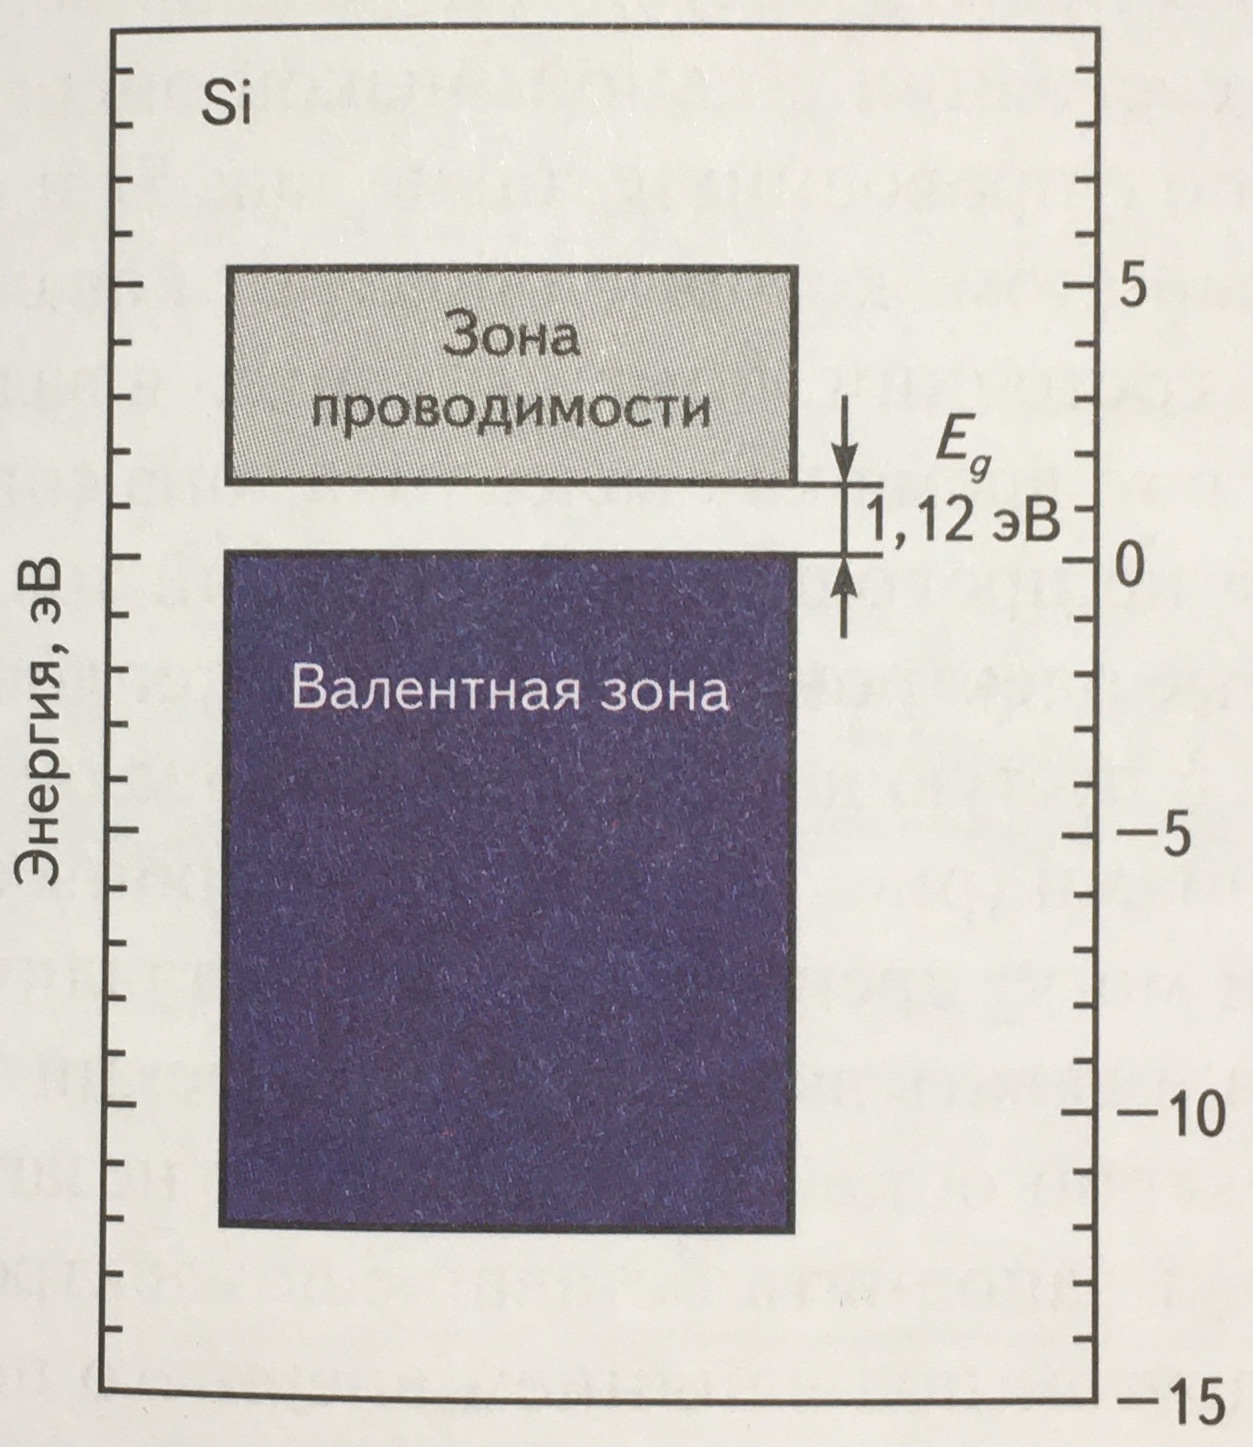
\includegraphics[width=\linewidth]{1}
    \caption{Энергетические зоны в Si, $E_{g}$ --- запрещенная зона,
    которая разделяет валентную зону и зону проводимости}
    \label{fig:1}
\end{wrapfigure}

Атомы, образующие твердые материалы, испытывают настолько сильные
межатомные взаимодействия, что их нельзя рассматривать как отдельные
сущности. Их электроны проводимости не связаны с отдельным атомом, а
принадлежат всему коллективу атомов как целому. Решение уравнения
Шредингера для энергии электрона в периодическом потенциале,
создаваемом атомами кристаллической решетки, приводит к расщеплению
энергии атомных уровней и формированию энергетических зон. Каждая зона
содержит большое число плотно расположенных дискретных энергетических
уровней, совокупность которых хорошо аппроксимируется континуумом. Как
видно на \fig{fig:1}, валентная зона отделена от зоны проводимости
запрещенной зоной с шириной $E_{g}$.


Волновые функции электронов в полупроводнике перекрываются, так что
действует \emph{принцип запрета Паули}. Этот принцип требует, чтобы в
каждом квантовом состоянии находилось не более одного электрона. Как и
в атомах, состояния с самой низкой энергией заполняются первыми.

При $T=0\: К$ число квантовых состояний, помещающихся в валентной зоне,
таково, что все они заполнены, в то время как валентная зона
совершенно пуста. При этих условиях материал не проводит электрический
ток. Однако с ростом температуры некоторые электроны в
результате теплового возбуждения попадают из валентной зоны в пустую
до этого зону проводимости, которая изобилует незанятыми состояниями
\ffig{fig:2}. Эти электроны становиться подвижными носителями заряда и
могут дрейфовать по кристаллической решетке под действием внешнего
поля и давать вклад в электрический ток. Кроме того, покидая валентную
зону, электрон оставляет после себя незаполненное квантовое состояние,
которое могут заполнять оставшиеся электроны валентной зоны, меняясь
местами друг с другом под влиянием внешнего поля. Таким образом,
оставшиеся в валентной зоне электроны приходят в движение. Это
движение эквивалентно движению в противоположном направлении дырки,
оставленной покинувшим зону электроном. Эта дырка ведет себя как
положительный заряд $e$.

\begin{figure}[H]
    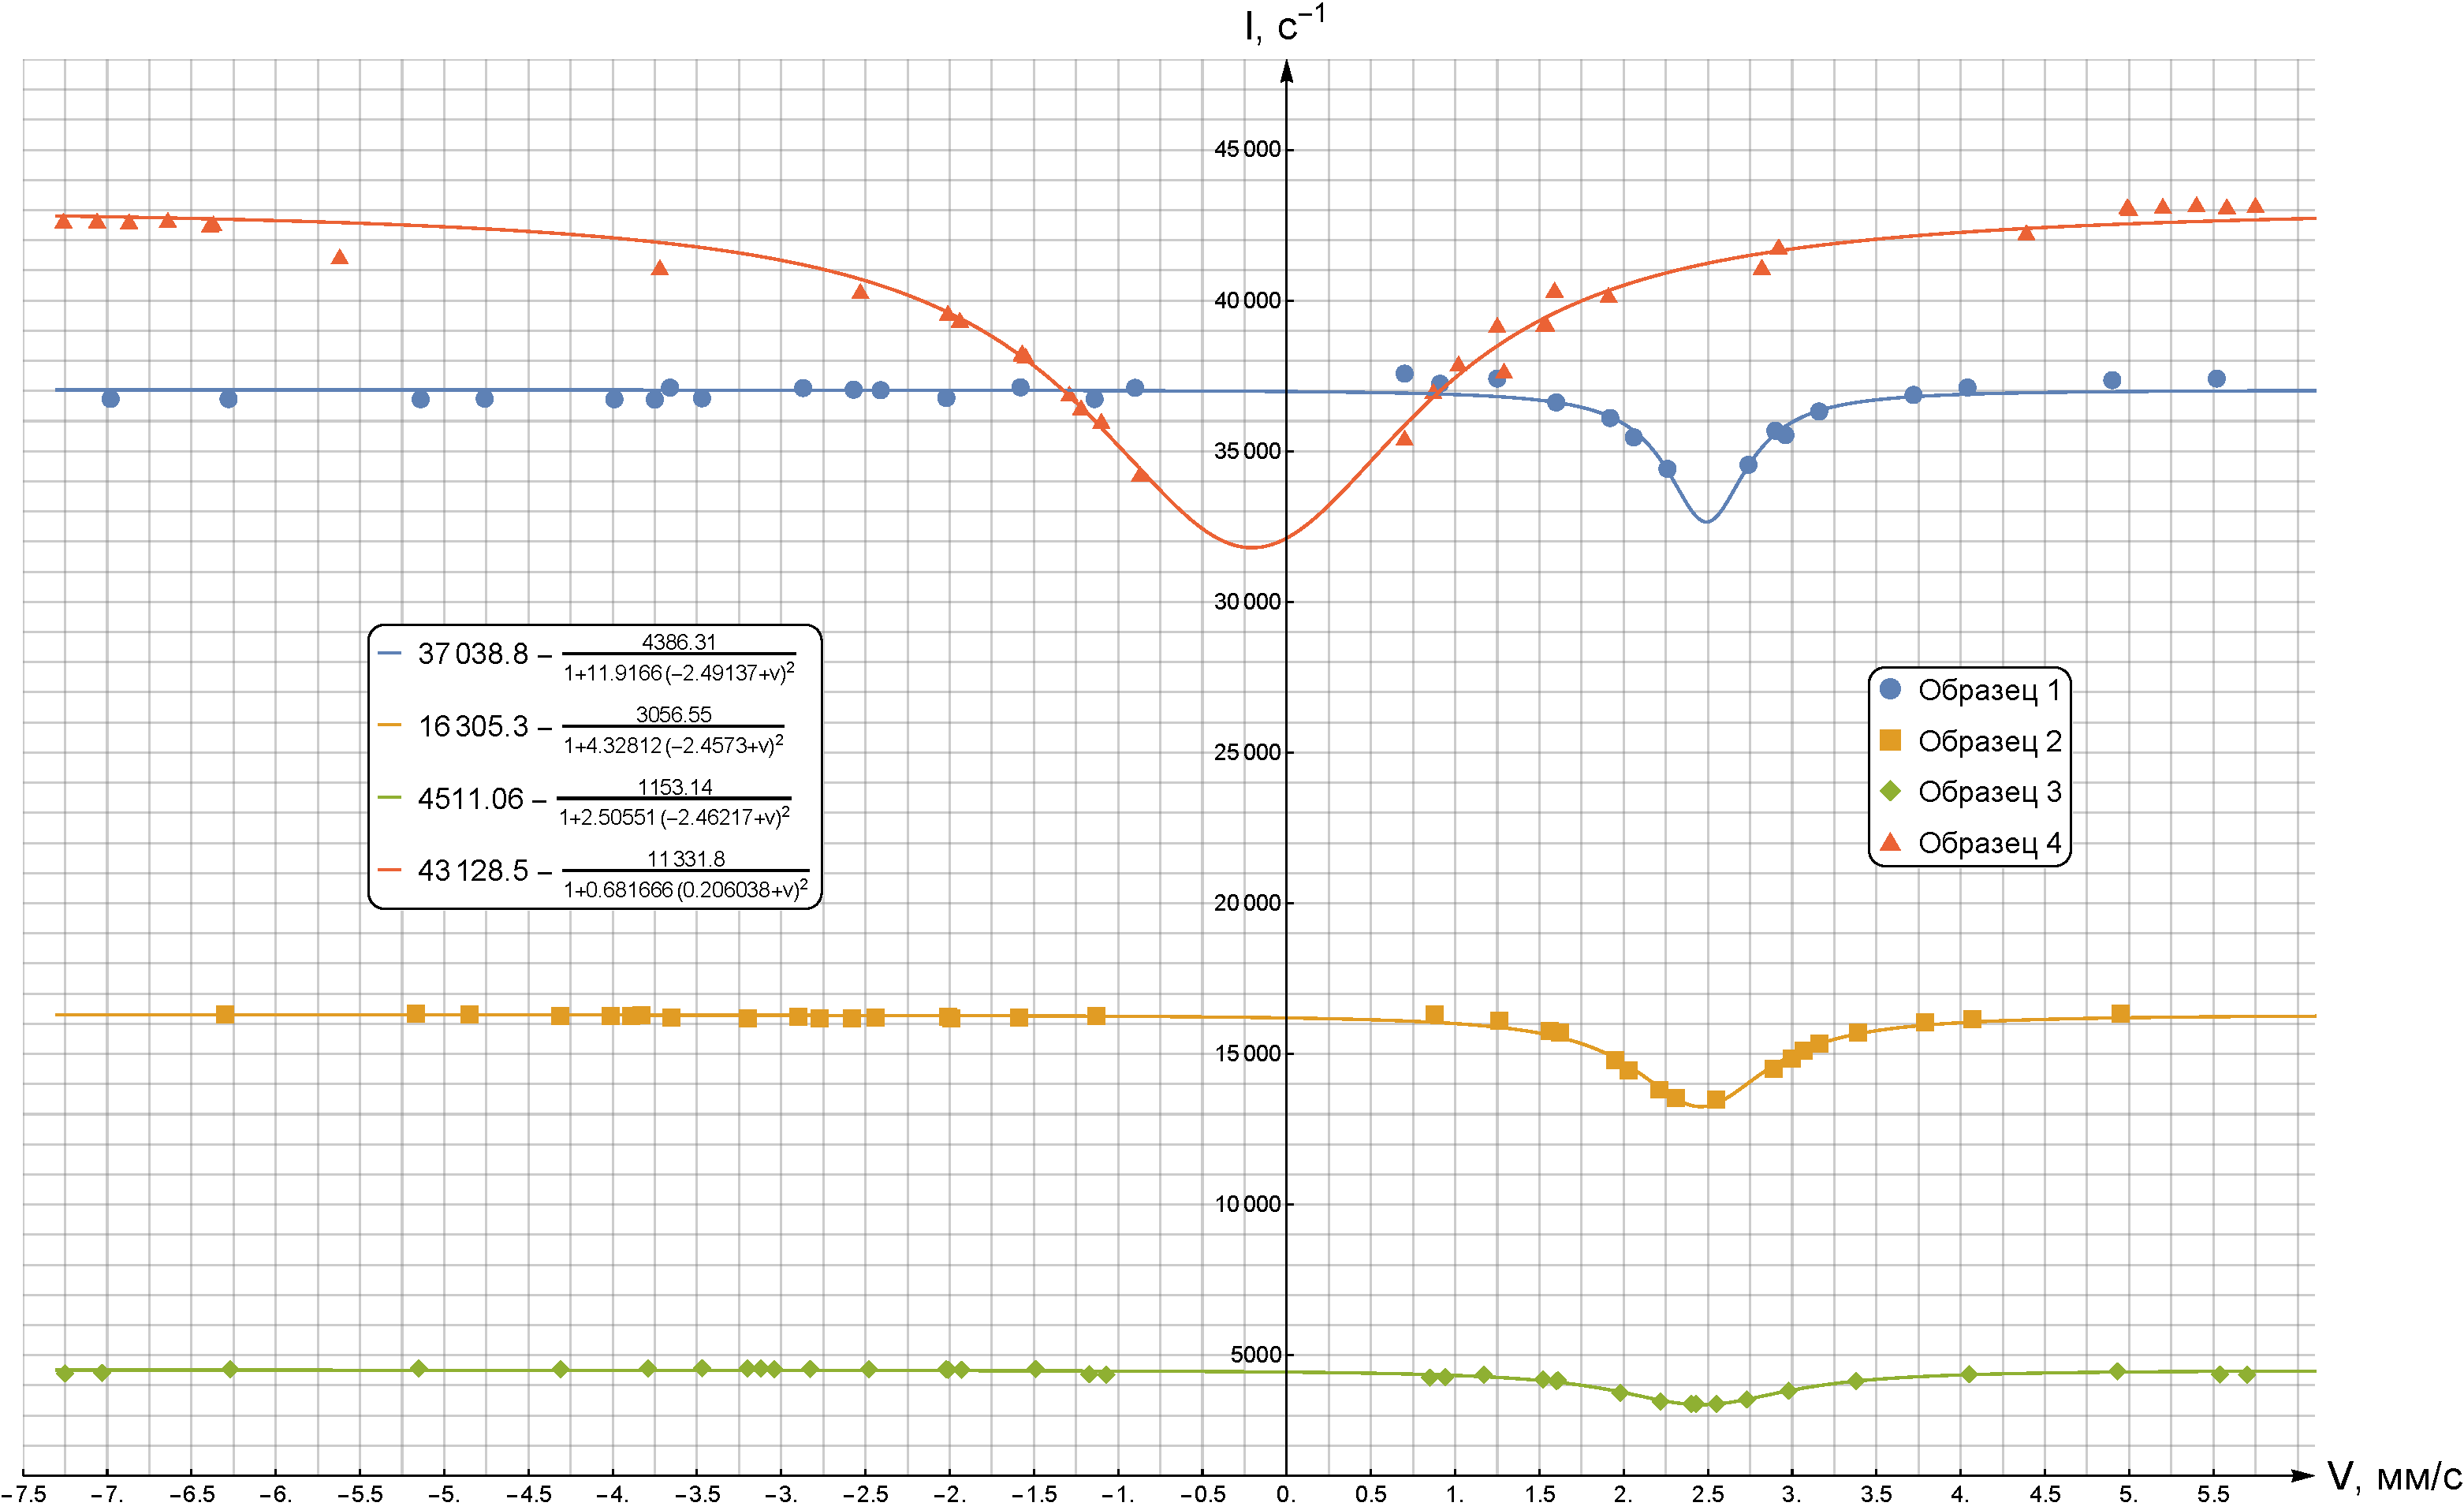
\includegraphics[width=0.55\linewidth]{2} 
    \caption{Электроны в зоне проводимости и дырки в валентной зоне
    при $T>0\: К$}
    \label{fig:2}
\end{figure}

В соответствии с волновой механикой энергия $E$ и импульс $p$
электрона в области постоянного потенциала, такой как свободное
пространство, связаны соотношением 
\begin{equation}
    E = \dfrac{p^2}{2m_{0}}=\dfrac{\hbar^2 k^2}{2m_{0}}
    \label{eq:1}
\end{equation}
где $p$ --- модуль импульса; $k$ --- модуль волнового вектора,
$k=p/\hbar$; $m_{0}$ --- масса электрона. Таким образом, соотношение
между $E$ и $k$ для свободного электрона --- простая параболическая
зависимость. Вблизи дна зоны проводимости зависимость $E$ от $k$ можно
аппроксимировать параболой 
\begin{equation}
    E = E_{c}+ \frac{\hbar^2 k^2}{2m_{c}}
    \label{eq:2}
\end{equation}

где $E_{c}$ --- энергия дна зоны проводимости; $k$ отсчитывается от
волнового вектора, при котором энергия имеет минимум. Это соотношение
показывает, что электрон зоны проводимости ведет себя так же, как
свободный электрон, но с массой $m_{c}$, которая называется
\emph{эффективной массой} электрона (в зоне проводимости) и отличается
от массы свободного электрона $m_{0}$. Таким образом, влияние ионов
решетки на движение электрона в зоне проводимости содержится в
эффективной массе $m_{c}$. Аналогично вблизи потолка валентной зоны
имеем 
\begin{equation}
    E=E_{v}-\dfrac{\hbar^2 k^2}{2 m_{v}},
    \label{eq:3}
\end{equation}
где $E_{v}=E_{c}-E_{g}$ --- энергия потолка валентной зоны; $m_{v}$
--- эффективная масса дырки (в валентной зоне). Влияние ионов решетки
на движение дырки в валентной зоне учитывается эффективной массой
$m_{v}$. Эффективная масса зависит от кристаллической структуры
материала и направления распространения по отношению к решетке,
поскольку межатомные расстояния различаются в разных
кристаллографических направлениях. Она также зависит от конкретной
рассматриваемой зоны.

Проводники, у которых минимум энергии в зоне проводимости и максимум
энергии в валентной зоне соответствуют одному и тому же значению
волнового числа $k$ (одинаковому импульсу), называются
\emph{прямозонными} материалами. Полупроводники, у которых это не так,
называются непрямозонными. Это различие важно, потому что переход
между дном зоны проводимости и потолком валентной зоны в непрямозонном
полупроводнике происходит с существенным изменением импульса
электрона. Прямозонные полупроводники являются эффективными
излучателями фотонов, а непрямозонные полупроводники не могут служить
эффективными излучателями света при обычных условиях.


\begin{figure}[H]
    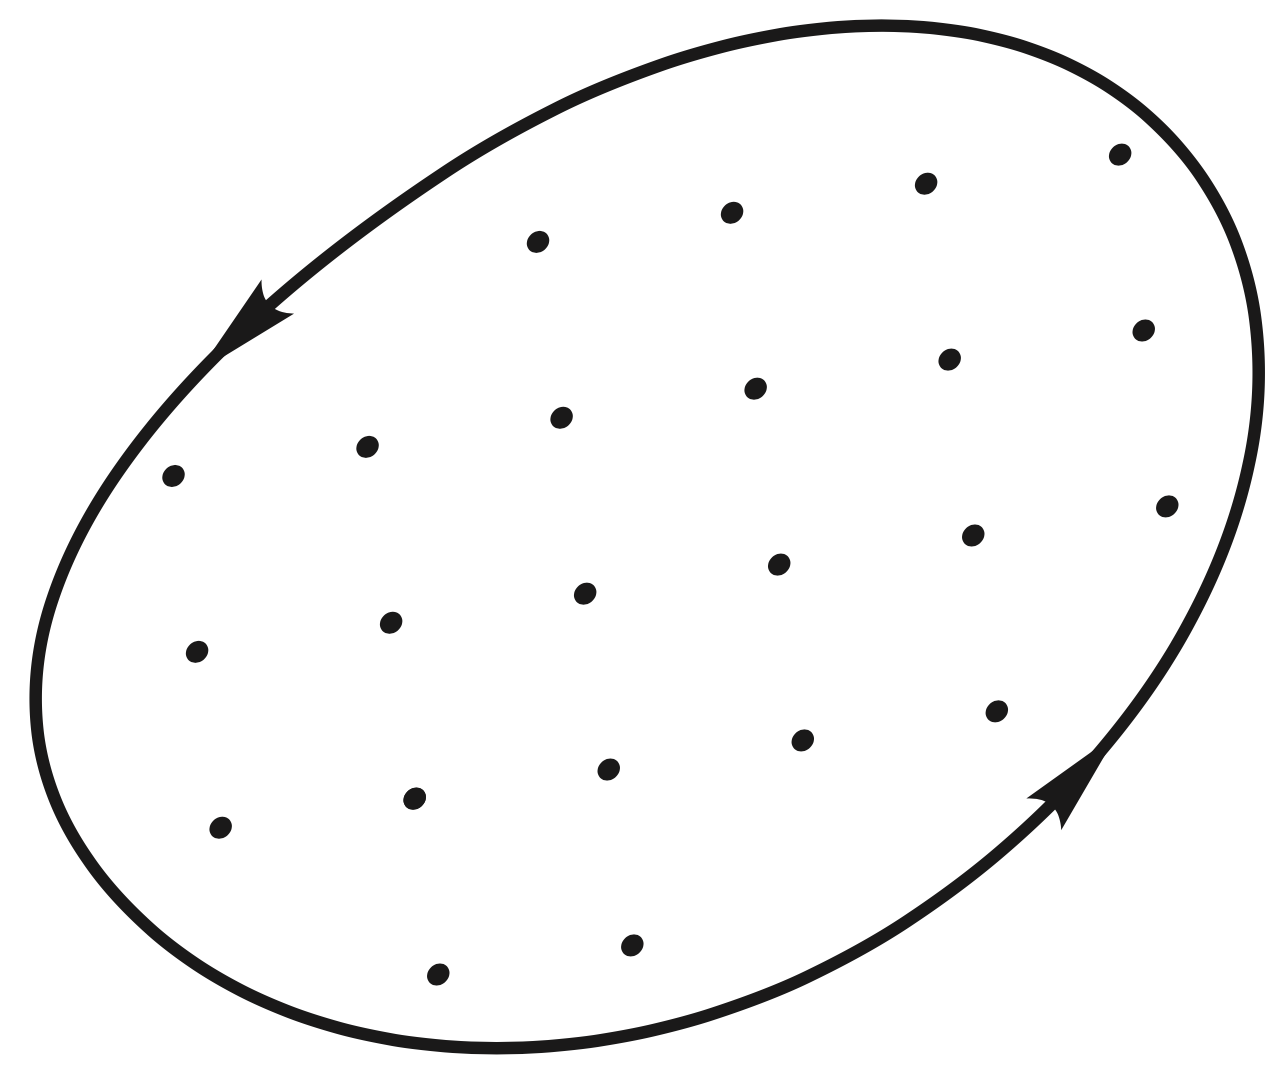
\includegraphics[width=0.8\linewidth]{3} 
    \caption{$E-k$-диаграммы для Si и GaAs хорошо аппроксимируются
    параболами вблизи дна зоны проводимости и потолка валентной зоны}
    \label{fig:3}
\end{figure}



\subsection{Примесные полупроводники}
Электрические и оптические свойства полупроводников могут существенно
меняться при контролируемом введении в материал небольшого
количества специально подобранных примесей или \emph{легирующих
добавок}. Введение примесей может изменить концентрацию подвижных
носителей заряда на много порядков величины. Легирующие добавки с
избытком валентных электронов, называемые \emph{донорами}, замещая
небольшое число нормальных атомов кристаллической решетки, создают
избыток подвижных электронов. В этом случае материал называется
\emph{полупроводником $n$-типа}. Аналогично, \emph{полупроводник
$p$-типа} получается при добавлении примесей с недостатком валентных
электронов, называемых \emph{акцепторами}. В результате получается
избыток свободных дырок. 

Полупроводники без умышленно введенных примесей называются
\emph{собственными} материалами, а с введением легирующих добавок ---
\emph{несобственными}.

\subsection{Концентрации электронов и дырок}
Определение концентрации носителей заряда в зависимости от энергии
требует знания двух характеристик --- плотности уровней энергии
(плотность состояний) и вероятности заселения каждого из этих уровней.

Квантовое состояние электрона в полупроводнике характеризуется его
энергией $E$, вектором $k$ и спином. Состояние описывается волновой
функцией, удовлетворяющей некоторым граничным условиям.

Вблизи края зоны проводимости электрон приближенно описывается как
частица массы $m_{c}$, находящаяся в трехмерном кубическом ящике
(размером $d$) c идеально отражающими стенками, т.е. в трехмерной
бесконечно глубокой прямоугольной потенциальной яме. Решения в виде
стоячих волн требуют, чтобы компоненты вектора
$\vec{k}=(k_{x},k_{y},k_{z})$ имели дискретные значения
$\vec{k}=(q_{1}\pi/d,q_{2}\pi /d,q_{3}\pi/d)$, где соответствующие
модовые числа $(q_{1},q_{2},q_{3})$ принимают целые положительные
значения. Этот результат является обобщением одномерной бесконечно
глубокой прямоугольной потенциальной ямы. Конец вектора $k$ должен
находиться в точках решетки, кубическая ячейка которой имеет размер
$\pi/d$. Таким образом, на единицу объема приходиться $(d/\pi)^3$
точек $\vec{k}$-пространстве. Число состояний, векторы $\vec{k}$
которых имеют модуль между $0$ и $k$, определяется подсчетом числа
точке, лежащих в положительном октанте сферы с радиусом $k$. В виду
наличия двух возможных спиновых состояний каждая точка в
$\vec{k}$-пространстве соответствует двум состояниям. Следовательно,
имеется приблизительно
\[
    2 \frac{\pi k^3/6}{(\pi/d)^3}= \frac{k^3}{3\pi^2}d^3
\]
таких точке в объеме $d^3$ и $(k^3/3\pi^2)$ точек в единичном объеме.
Отсюда следует, что число состояний с волновыми числами электрона
между $k$ и $k+\Delta k$, приходящееся на единичный объем,
\[
    \rho (k)\Delta k = \left( \frac{d}{dk}
    \frac{k^3}{3\pi^2}\right)\Delta k= \frac{k^2}{\pi^2}\Delta k,
\]
так что плотность состояний выражается как
\begin{equation}
    \rho(k) = \frac{k^2}{\pi^2}
    \label{eq:4}
\end{equation}

Если $\rho_{c}(E)\Delta E$ --- число энергетических уровней в зоне
проводимости (на единицу объема), лежащих между $E$ и $E+\Delta E$,
то, в силу взаимно однозначной связи \eqref{eq:2}  между $E$ и $k$, плотности
$\rho_{c}(E)$ и $\rho(k)$ должны быть связаны соотношением
$\rho_{c}(E)dE=\rho(k)dk$. Таким образом, плотность уровней энергии в
зоне проводимости равна 
\[
    \rho_{c}= \frac{\rho(k)}{dE/dk}.
\]
Аналогично, плотность состояний в валентной зоне 
\[
    \rho_{v}(E) = \frac{\rho(k)}{dE/dk},
\]
где $E$ дается формулой \eqref{eq:3}. Приближенные квадратичные
соотношения \eqref{eq:2} и \eqref{eq:3}, применимые вблизи краев зоны
проводимости и валентной зоны, соответственно, используются для
вычисления производной $dE/dk$ в каждой зоне. Результат получается
следующим
    \begin{align}
        \rho_{c}(E) = \frac{(2m_{c})^{3/2}}{2\pi^2
        \hbar^3}\sqrt{E-E_{c}},\hspace{1em} E \ge E_{c};\\
        \rho_{v}(E) = \frac{(2m_{c})^{3/2}}{2\pi^2
        \hbar^3}\sqrt{E_{v}-E},\hspace{1em} E \le E_{v}.
    \end{align}

Зависимость плотности состояний от энергии показана на \fig{fig:4}.
Она равна нулю на границе зоны и возрастает с удалением от нее со
скоростью, зависящей от эффективной массы электронов и дырок.


\begin{figure}[H]
    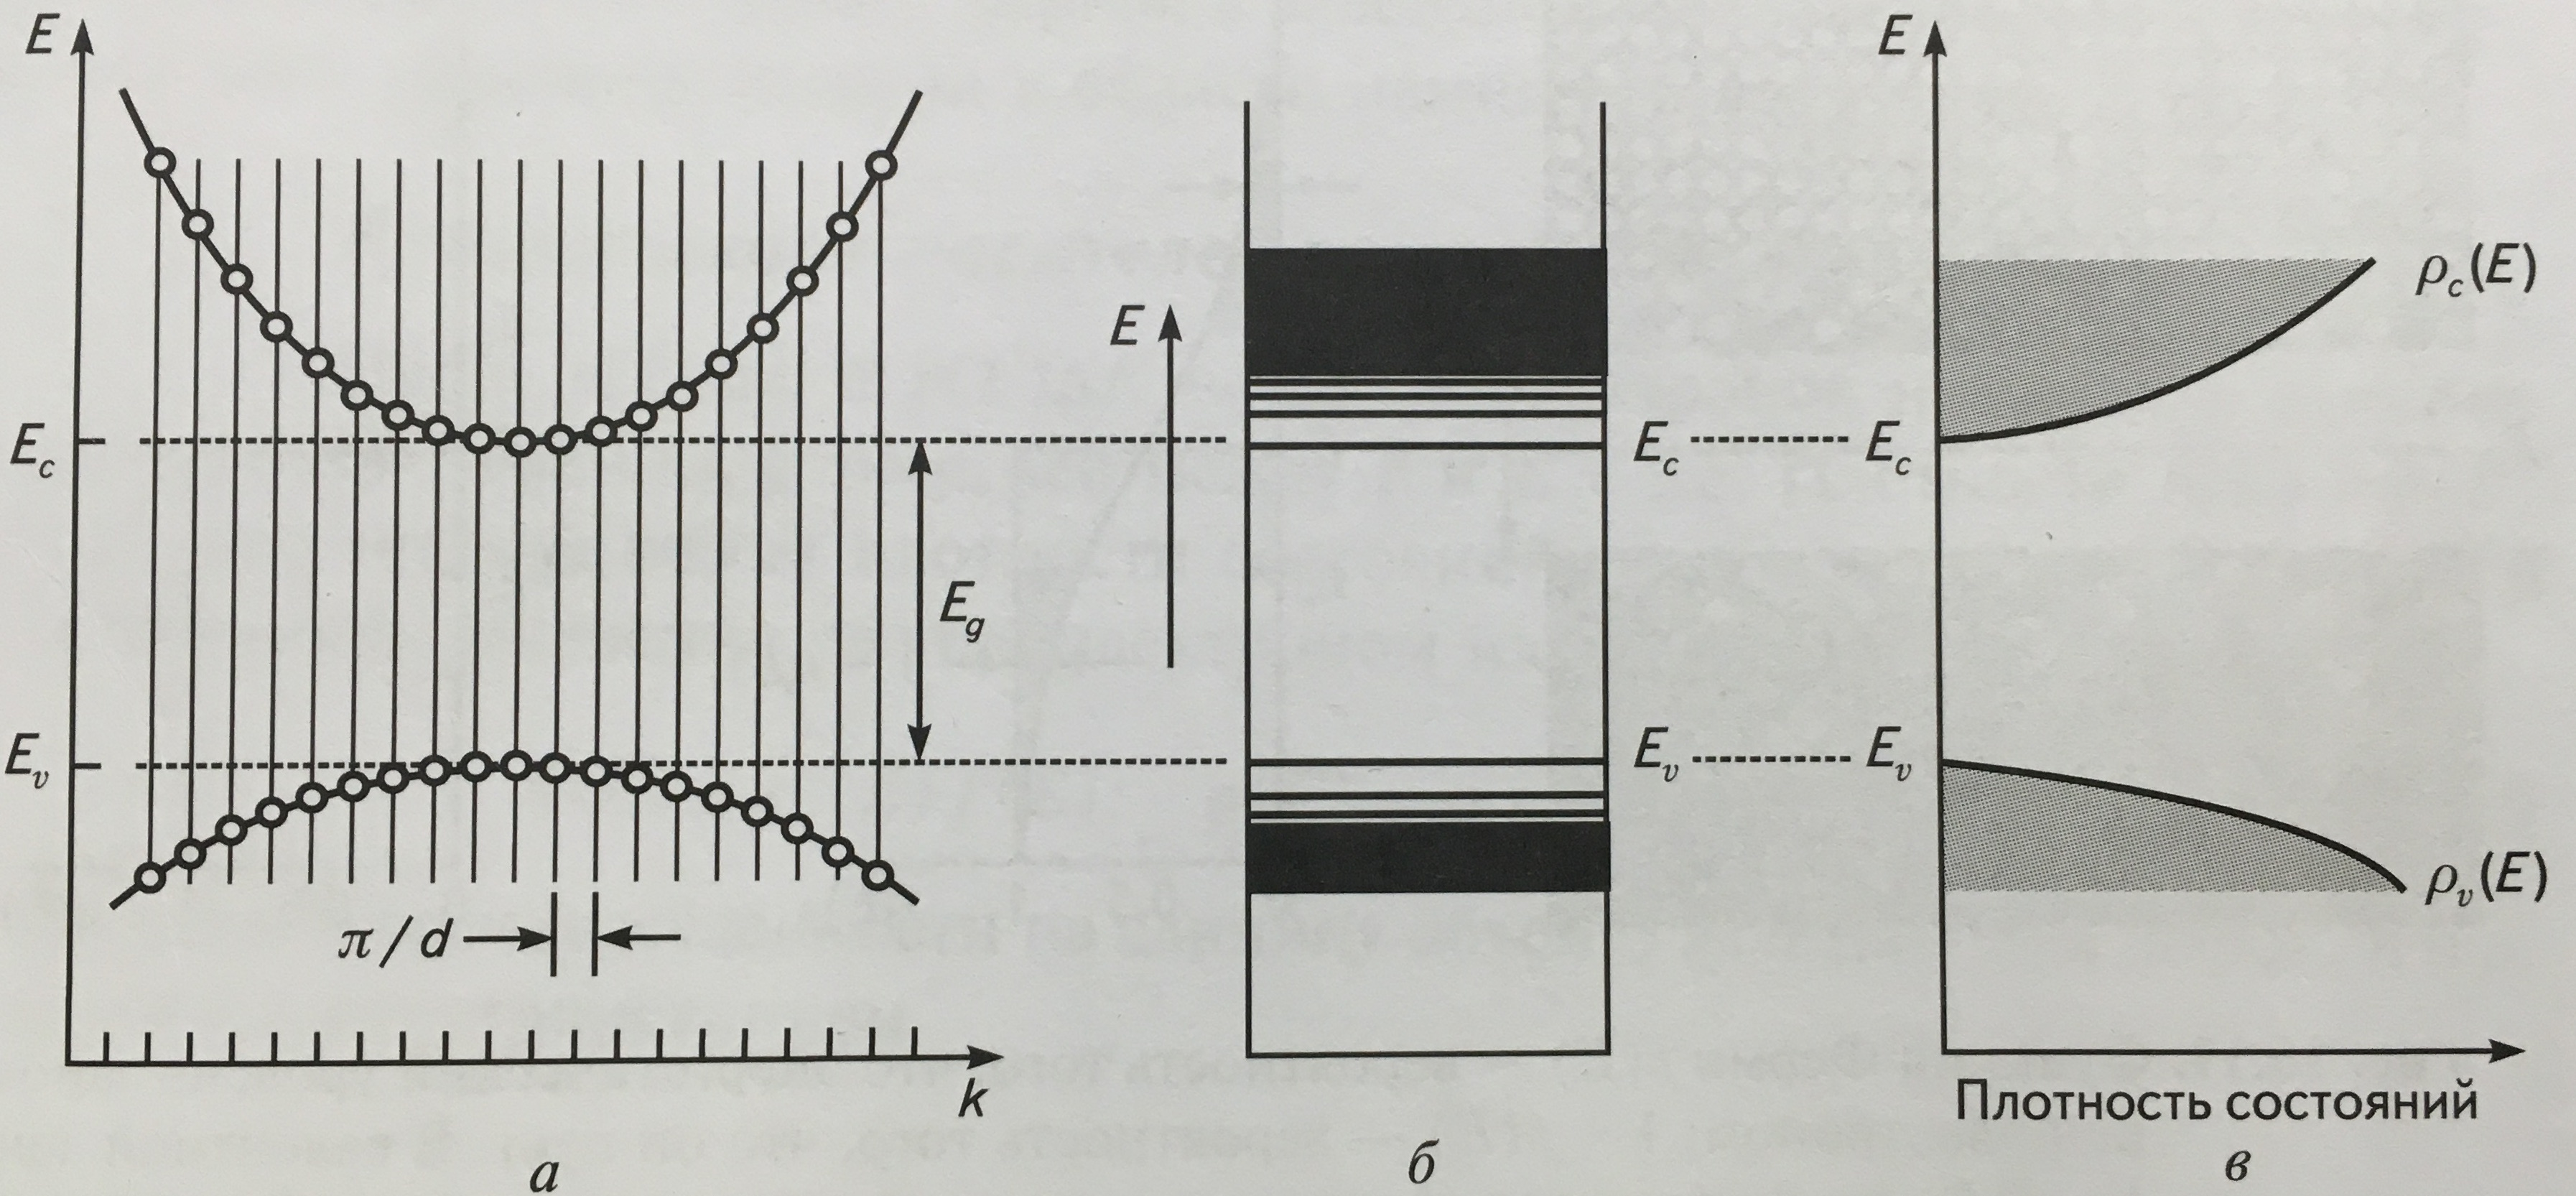
\includegraphics[width=0.7\linewidth]{4} 
    \caption{Зависимость $E$ от $k_{1}$ (при фиксированных $k_{2}$ и
    $k_{3}$) (a). Допустимые значения энергии (для всех $\vec{k}$)
(б). Плотность состояний вблизи краев зоны проводимости и валентной
зоны (в).}
\label{fig:4}
\end{figure}

В отсутствие теплового возбуждения (при $T=0\: K$) все электроны
занимают наинизшие возможные уровни энергии в соответствии с принципом
Паули. Валентная зона при этом полностью заполнена (нет дырок), а зона
проводимости полностью свободна (не содержит электронов). При
повышении температуры тепловое возбуждение переводит некоторые
электроны из валентной зоны в зону проводимости, оставляя в валентной
зоне свободные состояния (дырки). Из законов статистической механики
вытекает, что в состоянии теплового равновесия при температуре $T$
вероятность того, что данное состояние с энергией $E$ занято
электроном, определяется функцией Ферми
\begin{equation}
    f(E) = \frac{1}{\exp \left[\left(E-E_{f}\right)/k_{B}T\right]+1}
    \label{eq:7}
\end{equation}
где $k_{B}$ --- постоянная Больцмана; $E_{f}$ --- постоянная,
называемая \emph{энергией} или \emph{уровнем} \emph{Ферми}. Функция
\eqref{eq:7} называется также \emph{распределением Ферми-Дирака}.
Каждый энергетический уровень $E$ либо занят (с вероятностью $f(E)$),
либо пусть (c вероятностью $1-f(E)$). Вероятности $f(E)$ и $1-f(E)$
зависят от энергии $E$, согласно формуле \eqref{eq:7}. Функция $f(E)$
не является плотностью вероятности, и ее интеграл по всем $E$ не равен
единице. Она дает последовательность вероятностей заселения следующих
друг за другом уровней энергии.


\begin{figure}[H]
    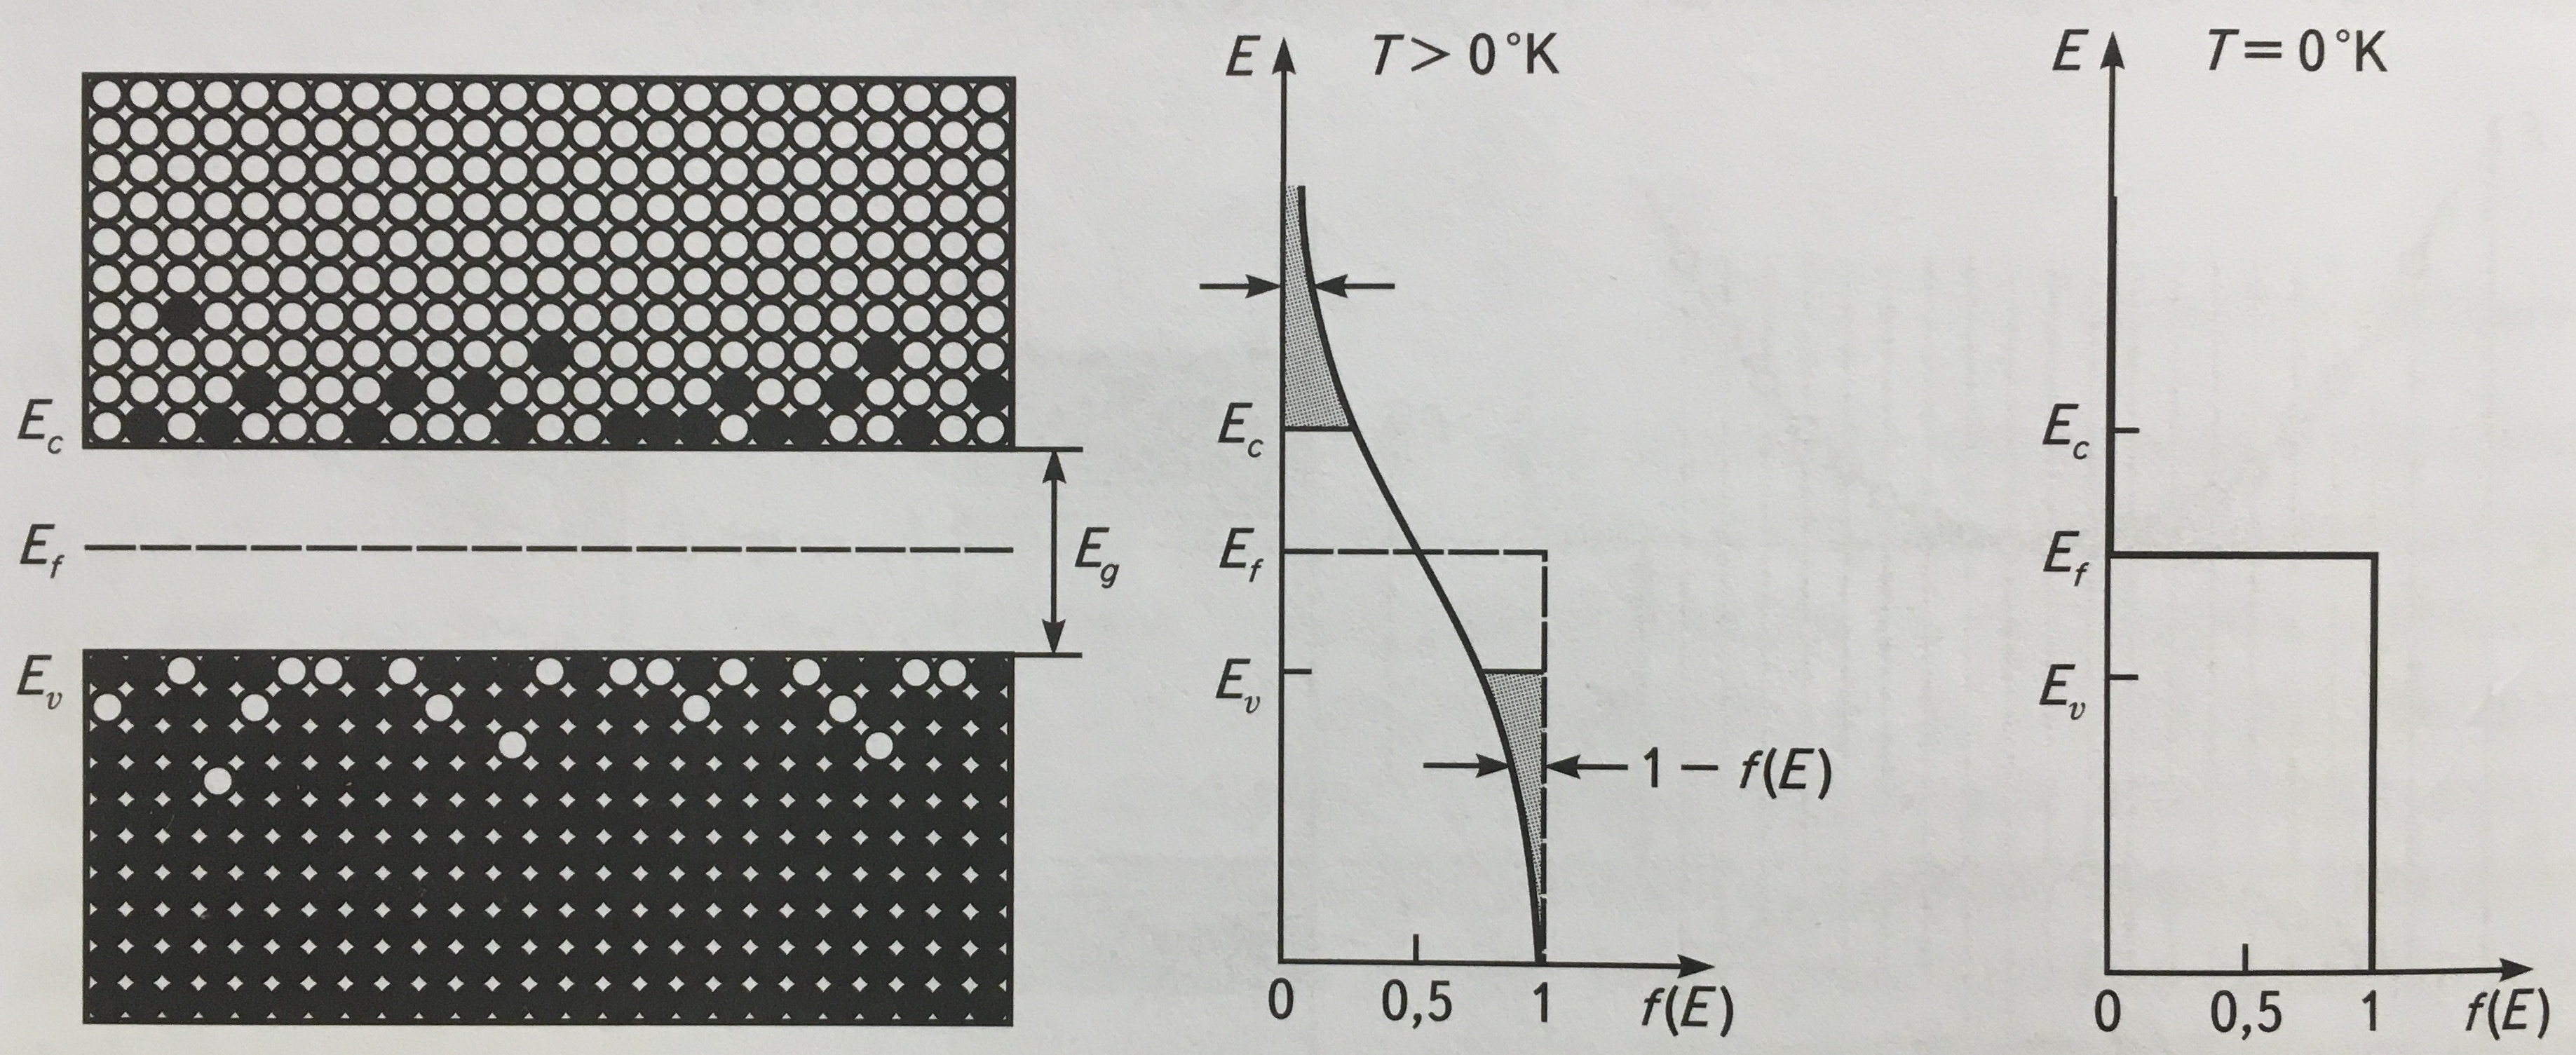
\includegraphics[width=0.7\linewidth]{5} 
    \caption{Функция Ферми $f(E)$}
    \label{fig:5}
\end{figure}

Поскольку $f(E_{f}) = 1/2$, какой бы ни была температура $T$, уровень
Ферми представляет собой ту энергию, при которой вероятность заселения
энергетического уровня (если такой уровень существует) равна 1/2.
Функция Ферми монотонно убывает с ростом энергии $E$. При $T=0\: К$ 
$f(E)=0,$ если $E>E_{f}$, и $f(E)=1$, если $E\le E_{f}$. Этим
определяется физический смысл $E_{f}:$ это энергия, отделяющая
заселенные уровни от незаселенных при $T=0\: К$. Поскольку $f(E)$ ---
вероятность того, что уровень заселен, есть вероятность того, что он
пусть, то $1-f(E)$ есть вероятность того, что уровень занят дыркой,
если он лежит в валентной зоне. 

Эти функции симметричны относительно уровня Ферми. Когда $E-E_{f}\gg
k_{B}T,$
\[
    f(E)\approx \exp \left[- \frac{E-E_{f}}{k_{B}T}\right].
\]
Тогда функция Ферми пропорциональная распределению Больцмана, которое
описывает экспоненциальную энергетическую зависимость доли общего
числа атомов, приходящейся на данный энергетический уровень. Из
соображений симметрии вытекает, что когда $E<E_{f}$ и $E_{f}-E \gg
k_{B}T$,
\[
    1-f(E) \approx \exp \left[- \frac{E_{f}-E}{k_{B}T}\right];
\]
вероятность заселения уровня дыркой в валентной зоне экспоненциально
затухает по мере убывания энергии в области намного ниже уровня Ферми.

\subsection{Рекомбинация}
Тепловое возбуждение электронов с переходом из валентной зоны в зону
проводимости приводит к \emph{электронно-дырочной генерации}. Тепловое
равновесие требует, чтобы генерация сопровождалась одновременным
обратным процессом ликвидации возбуждения; Этот процесс, называемый
\emph{электронно-дырочной рекомбинацией}, характеризуется переходом
электрона из зоны проводимости в валентную зону с заполнением дырки.
Энергия электрона при этом может высвобождаться в виде испущенного
фотона, тогда процесс называется \emph{радиационной
рекомбинацией}.

Безызлучательная рекомбинация может происходить за счет целого ряда
независимых конкурирующих процессов, включающих передачу энергии
колебаниям решетки или другому свободному электрону (процесс Оже).
Рекомбинация может происходить на поверхности, а также непрямым путем
через ловушки --- энергетические уровни, связанные с примесями,
границами зерен, дислокациями или другими нарушениями структуры
решетки и лежащие внутри запрещенной зоны. Примесь или дефект может
вести себя как центр рекомбинации, если он способен захватывать
электроны и дырки одновременно, увеличивая вероятность их
рекомбинации. Примесная рекомбинация может быть радиационной или
безызлучательной. 

\subsection{Переходы}
Соединения областей с различным легирование в одном полупроводниковом
материале называются \emph{гомопереходами}. Важным примером является
$p-n$-перехода. Переходы мжеду различными полупроводниковыми
материалами называются \emph{гетеропереходами}. 

$p-n$-переход состоит из контактирующих областей $p-$ и $n-$ типа в
одном и том же полупроводнике. Область $p$-типа имеет большое
количество дырок (основных носителей) и мало подвижных электронов
(неосновных носителей). В области $n$-типа много подвижных электронов
и мало дырок. Оба типа носителей заряда находятся в непрерывном
тепловом движении во всех направлениях.

Когда две области приводятся в контакт друг с другом, происходит
следующее:
\begin{itemize}
    \item Электроны и дырки диффундируют из области высокой
        концентрации в область низкой. Электроны диффукндируют из
        $n$-области в $p$-область, оставляя после себя положительно
        заряженные ионизированные атомы донора. В $p$-области
        электроны рекомбинируют с дырками, которых там много.
        Аналогично, дырки диффундируют из $p$-области в $n$-область,
        оставляя за собой отрицательно заряженные ионизированные атомы
        акцептора. В $n$-области дырки рекомбинируют с подвижными
        электронами, которыми она богата. Однако этот процесс диффузии
        не продолжается бесконечно, поскольку он вызывает нарушение
        баланса зарядов в обеих областях.
    \item В результате узкая область по обе стороны перехода
        становится почти лишенной подвижных носителей заряда. Эта
        область называется \emph{обедненным слоем}. Он содержит только
        неподвижные заряда (положительные ионы со стороны $n$-области
        и отрицательные --- со стороны $p$-области). Толщина
        обедненного слоя в каждой области обратно пропорциональна
        концентрации соответствующей примени в ней.
    \item Неподвижные заряда создают электрическое поле в обедненном
        слое, направленное из $n$-области в $p$-область. Это поле
        препятствует дальнейшей диффузии подвижных носителей заряда
        через переход.
    \item Устанавливается равновесие, результатом которого является
        возникновение разности потенциалов $V_{0}$ между двумя
        сторонами обедненного слоя, причем потенциал со стороны
        $n$-области выше, чем со стороны $p$-области.
    \item Из-за указанной разности потенциалов потенциальная энергия
        электрона со стороны $n$-области ниже, чем со стороны
        $p$-области. В результате этого энергетические зоны
        изгибаются, как показано на \fig{fig:6}. В состоянии теплового
        равновесия существует единственная функция Ферми для всей
        структуры, поэтому уровни Ферми в $n$- и $p$-областях должны
        совпадать.
    \item Полный ток через переход равен нулю. Токи, связанные с
        диффузией, и токи, вызванные разностью потенциалов (дрейфовые
        токи), компенсируют друг друга как для электронов, так и для
        дырок.
\end{itemize}


\begin{figure}[H]
    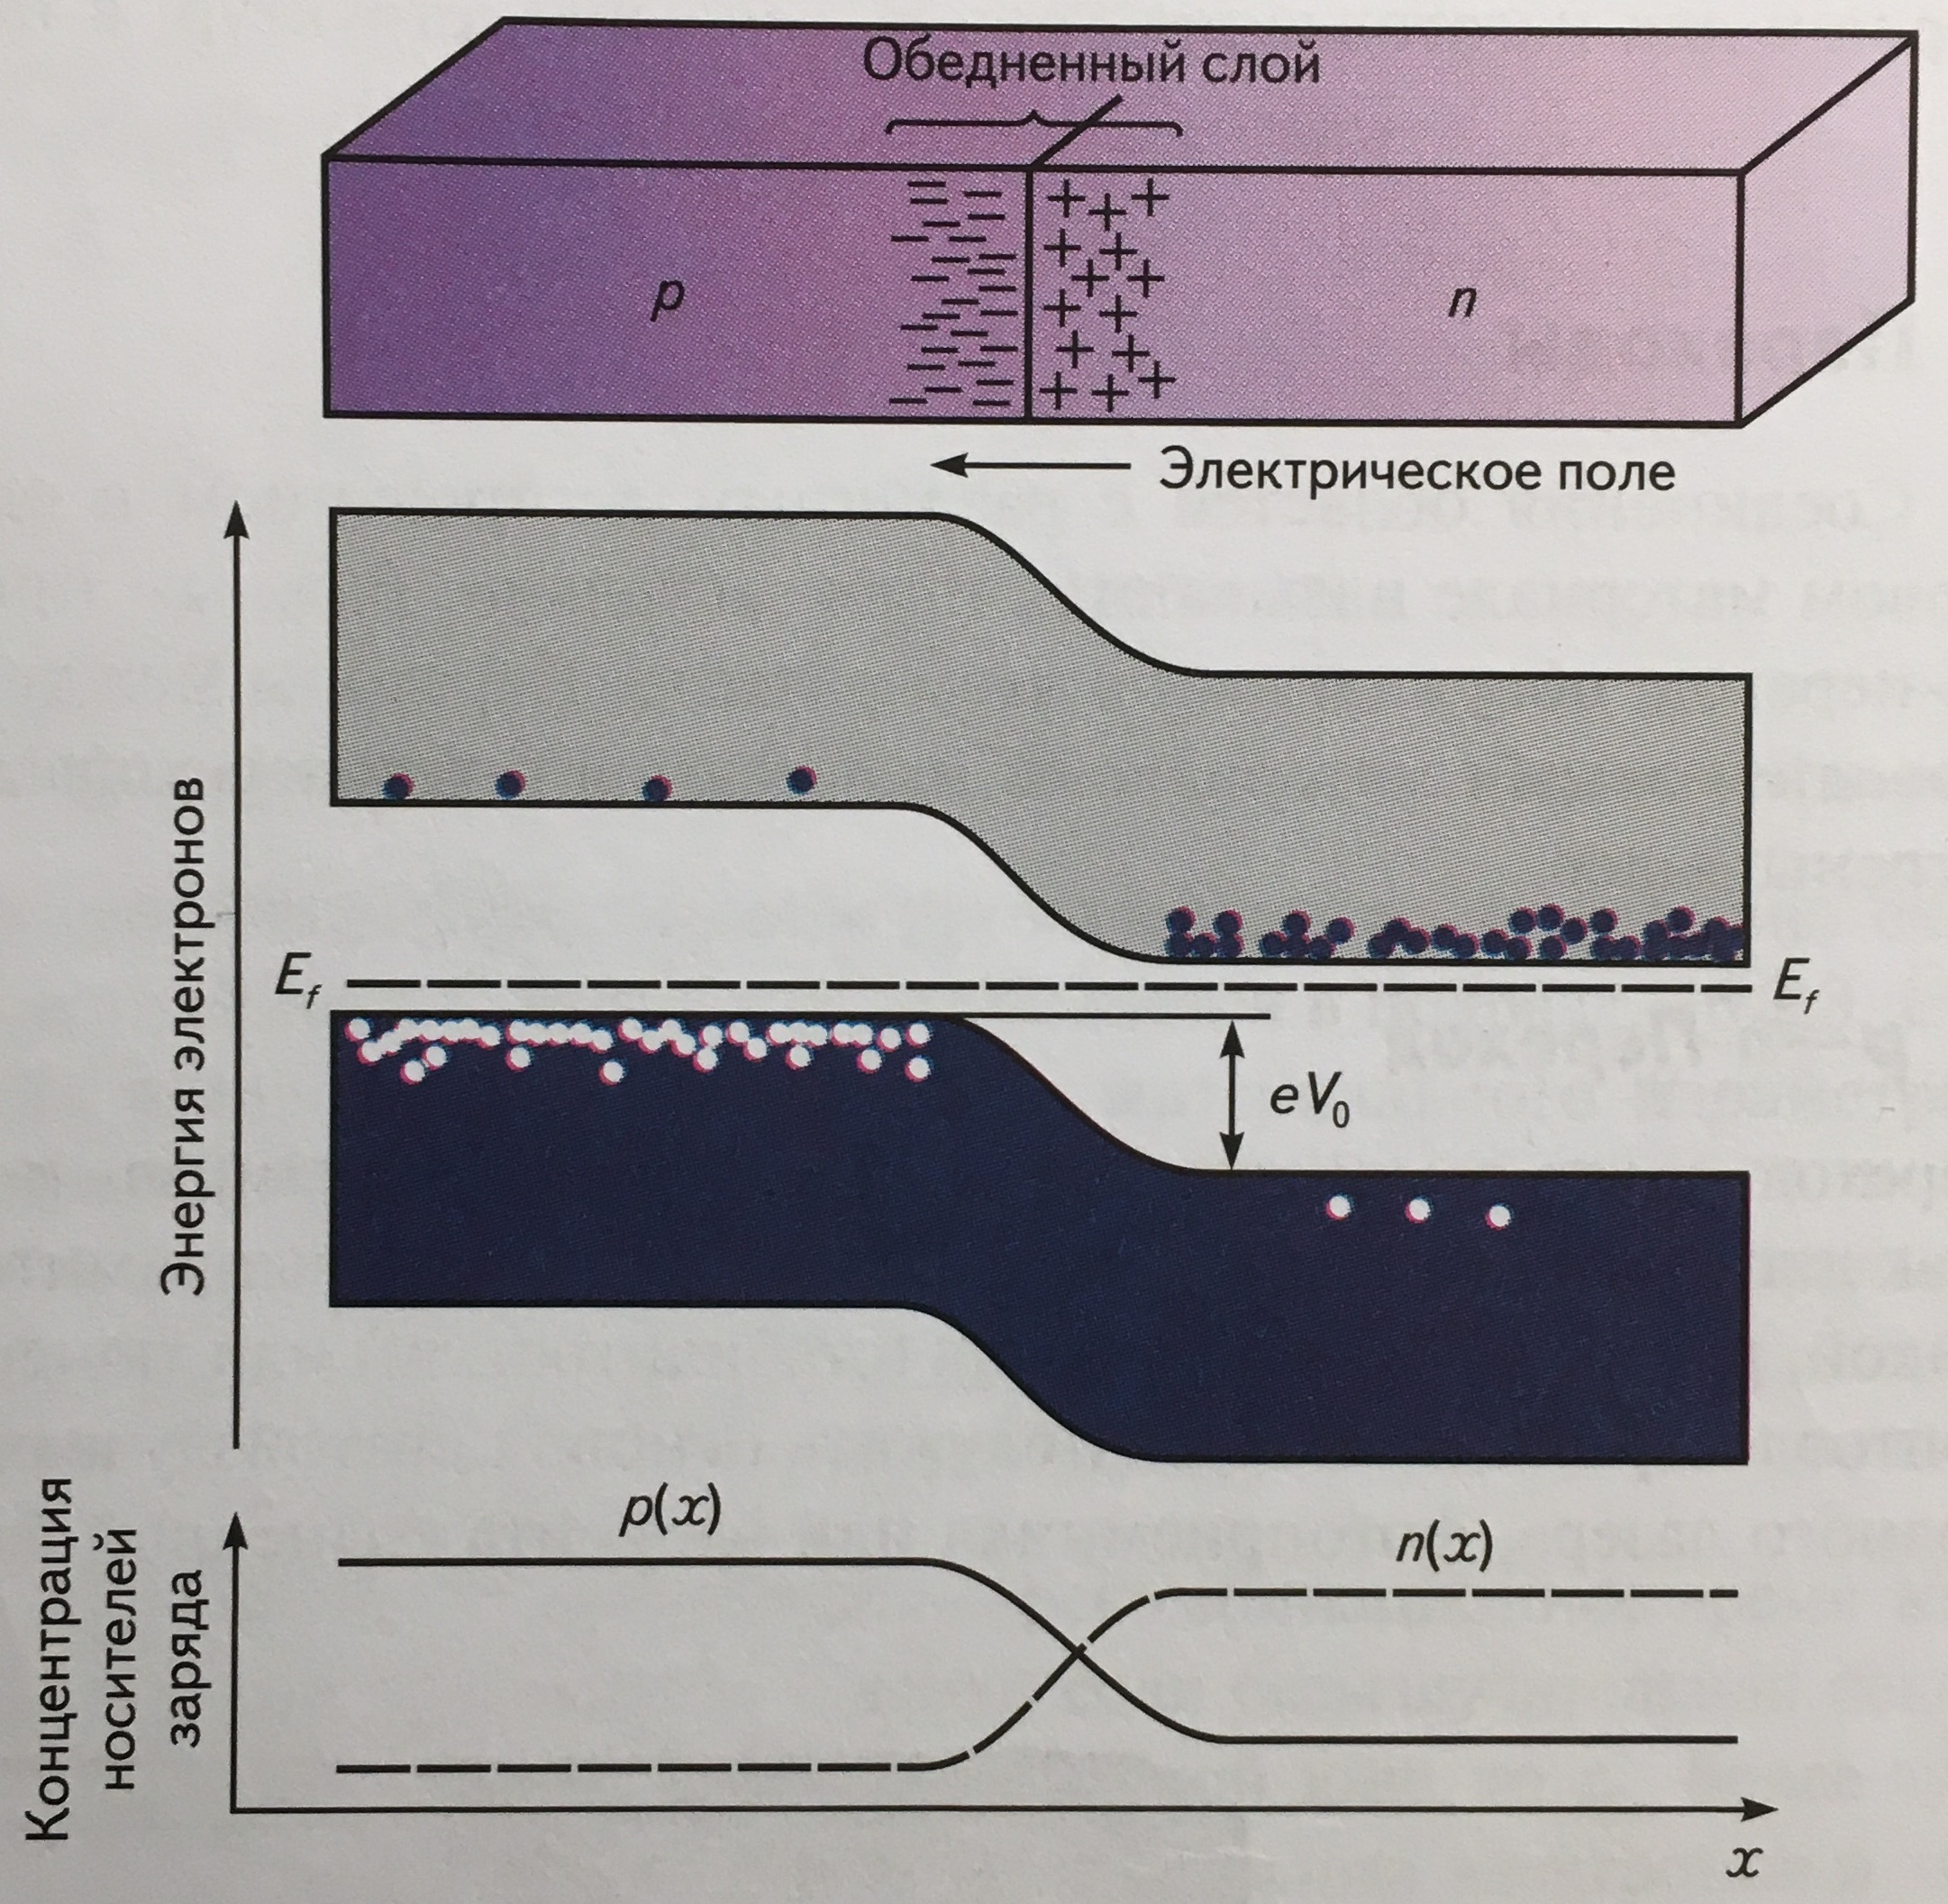
\includegraphics[width=0.7\linewidth]{6} 
    \caption{$p-n$ переход в состоянии теплового равновесия при $T>0\:
    К$. Обедненный слой, схема энергитических зон и концентрации (в
логарифмической шкале) подвижных электронов $n(x)$ и дырок $p(x)$
показаны в зависимости от координаты $x$. Контактная разность
потенциалов $V_{0}$ соответствует энергии $eV_{0}$, где $e$---
величина заряда электрона}
\label{fig:6}
\end{figure}



Приложенный извне потенциал изменяет разность потенциалов между $p-$ и
$n$-областями. Это, в свою очередь, меняет поток основных носителей,
так что переход может действовать как <<затвор>>. Если переход
подвергается \emph{прямому смещению} путем приложения положительного
напряжения $V$ к $p$-области, то ее потенциал увеличивается
относительно $n$-области, так что электрическое поле создается в
направлении, противоположном собственному полю $p-n$-перехода.
Присутствие внешнего смещающего напряжения вызывает выход из состояния
равновесия и рассогласование уровней Ферми в $p-$ и $n$-областях, а
также в обедненном слое. Наличие двух уровней Ферми в $E_{fc}$ и
$E_{fv}$ в обедненном слове представляет состояние квазиравновесия.

Полный эффект от прямого смещения состоит в понижении потенциальной
ступени на величину $eV$. Ток основных носителей возрастает в
$\exp(eV/k_{B}T)$ раз, так что полный ток становится равным
\[
    i=i_{s}\exp \left( \frac{eV}{k_{B}T}\right)-i_{s},
\]
где $i_{s}$ --- постоянная величина. Избыточные основные носители ---
дырки и электроны, которые попадают в $n-$ и $p-$области,
соответственно, становятся неосновными носителями и рекомбинируют с
местными основными носителями. Поэтому их концентрация убывает с
увеличением расстояния до перехода, как показано на \fig{fig:7}. Этот
процесс называется \emph{инжекцией неосновных носителей}.  

При обратном смещении перехода путем приложения отрицательного
напряжения $V$ к $p$-области высота потенциальной ступени
увеличивается на $eV$. Это препятствует потоку основных носителей.
Соответствующий ток умножается на $\exp (eV/k_{B}T)$, где $V$
отрицательно, т.е. уменьшается. Полный ток становится равным
$i=i_{s}\exp(eV/k_{B}T)-i_{s}$, так что небольшой ток $\approx i_{s}$
течет в обратном направлении при $|V|\gg k_{B}T/e$.


\begin{figure}[H]
    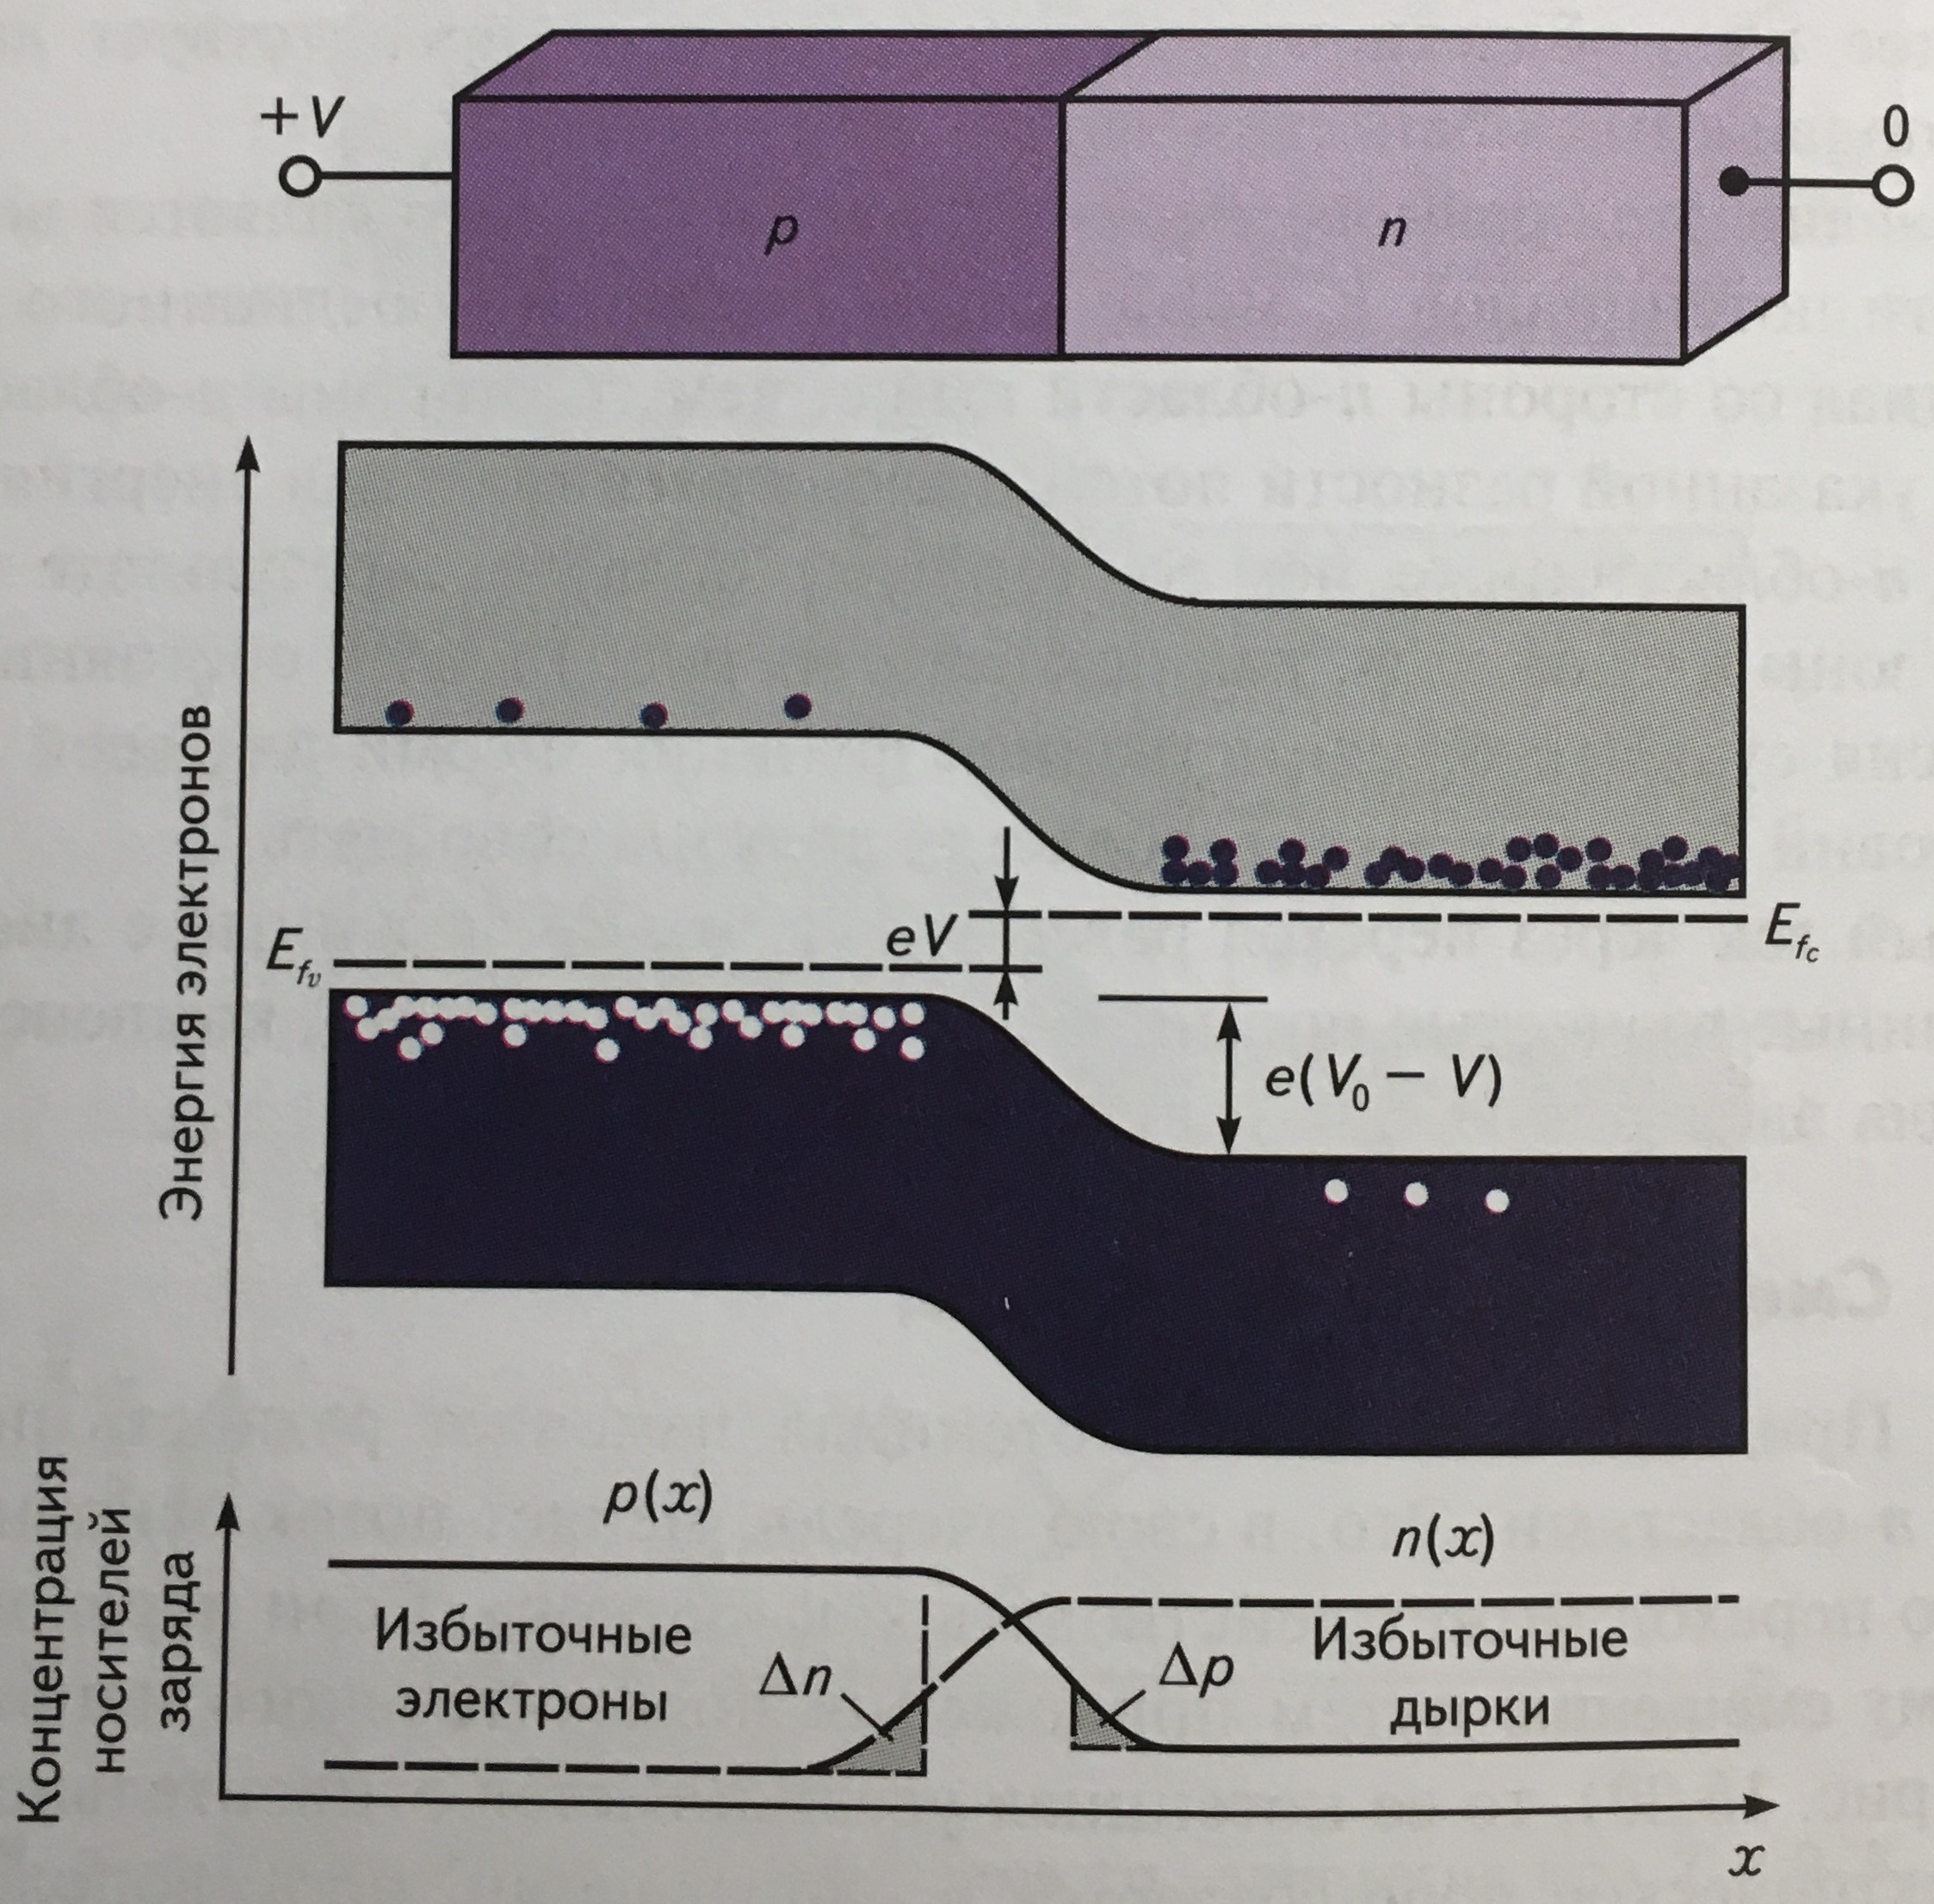
\includegraphics[width=0.65\linewidth]{7} 
    \caption{Схема энергетических зон и концентрация носителей для
    $p-n$-перехода, смещенного в прямом направлении}
    \label{fig:7}
\end{figure}

Таким образом, $p-n$-переход действует как диод с вольт-амперной
характеристикой 
\begin{equation}
    i=i_{s} \left[\exp \left( \frac{eV}{k_{B}T}\right)-1\right].
    \label{eq:diod}
\end{equation}
Характеристика идеального диода известна как уравнение Шокли.

Контакт различных полупроводников может иметь некоторые преимущества по
сравнению с контактом одинаковых полупроводников:
\begin{itemize}
    \item Переход между материалами с различной шириной запрещенной
        зоны создает локальный скачок зонной структуры. Разрыв
        потенциальной энергии создает барьер, который может быть
        полезным для предотвращения проникновения определенного типа
        носителей в области, где их присутствие нежелательно. Это
        свойство может быть использовано, например, в $p-n$-переходе
        для уменьшения части тока, переносимого неосновными
        носителями, и, следовательно, для повышения эффективности
        инжекции.
    \item Разрывы энергетических зон, создаваемые двумя
        гетеропереходами, могут быть полезны для удержания носителей
        заряда в заданной области пространства. Например, слой
        материала с узкой запрещенной зоной можно поместить между
        двумя слоями материалов с большей шириной запрещенной зоны,
        как в $p-p-n$-структуре, показанной на \fig{fig:8} и состоящей
        из гетеропереходов $p-p$ и $p-n$. Такая \emph{двойная
        гетероструктура}  эффективно используется при изготовлении
        светодиодов, полупроводниковых усилителей света и диодных
        лазеров.
    \item гетеропереходы полезны для создания разрывов энергетических
        зон, которые ускоряют носители заряда в нужных местах.
\end{itemize}


\begin{figure}[H]
    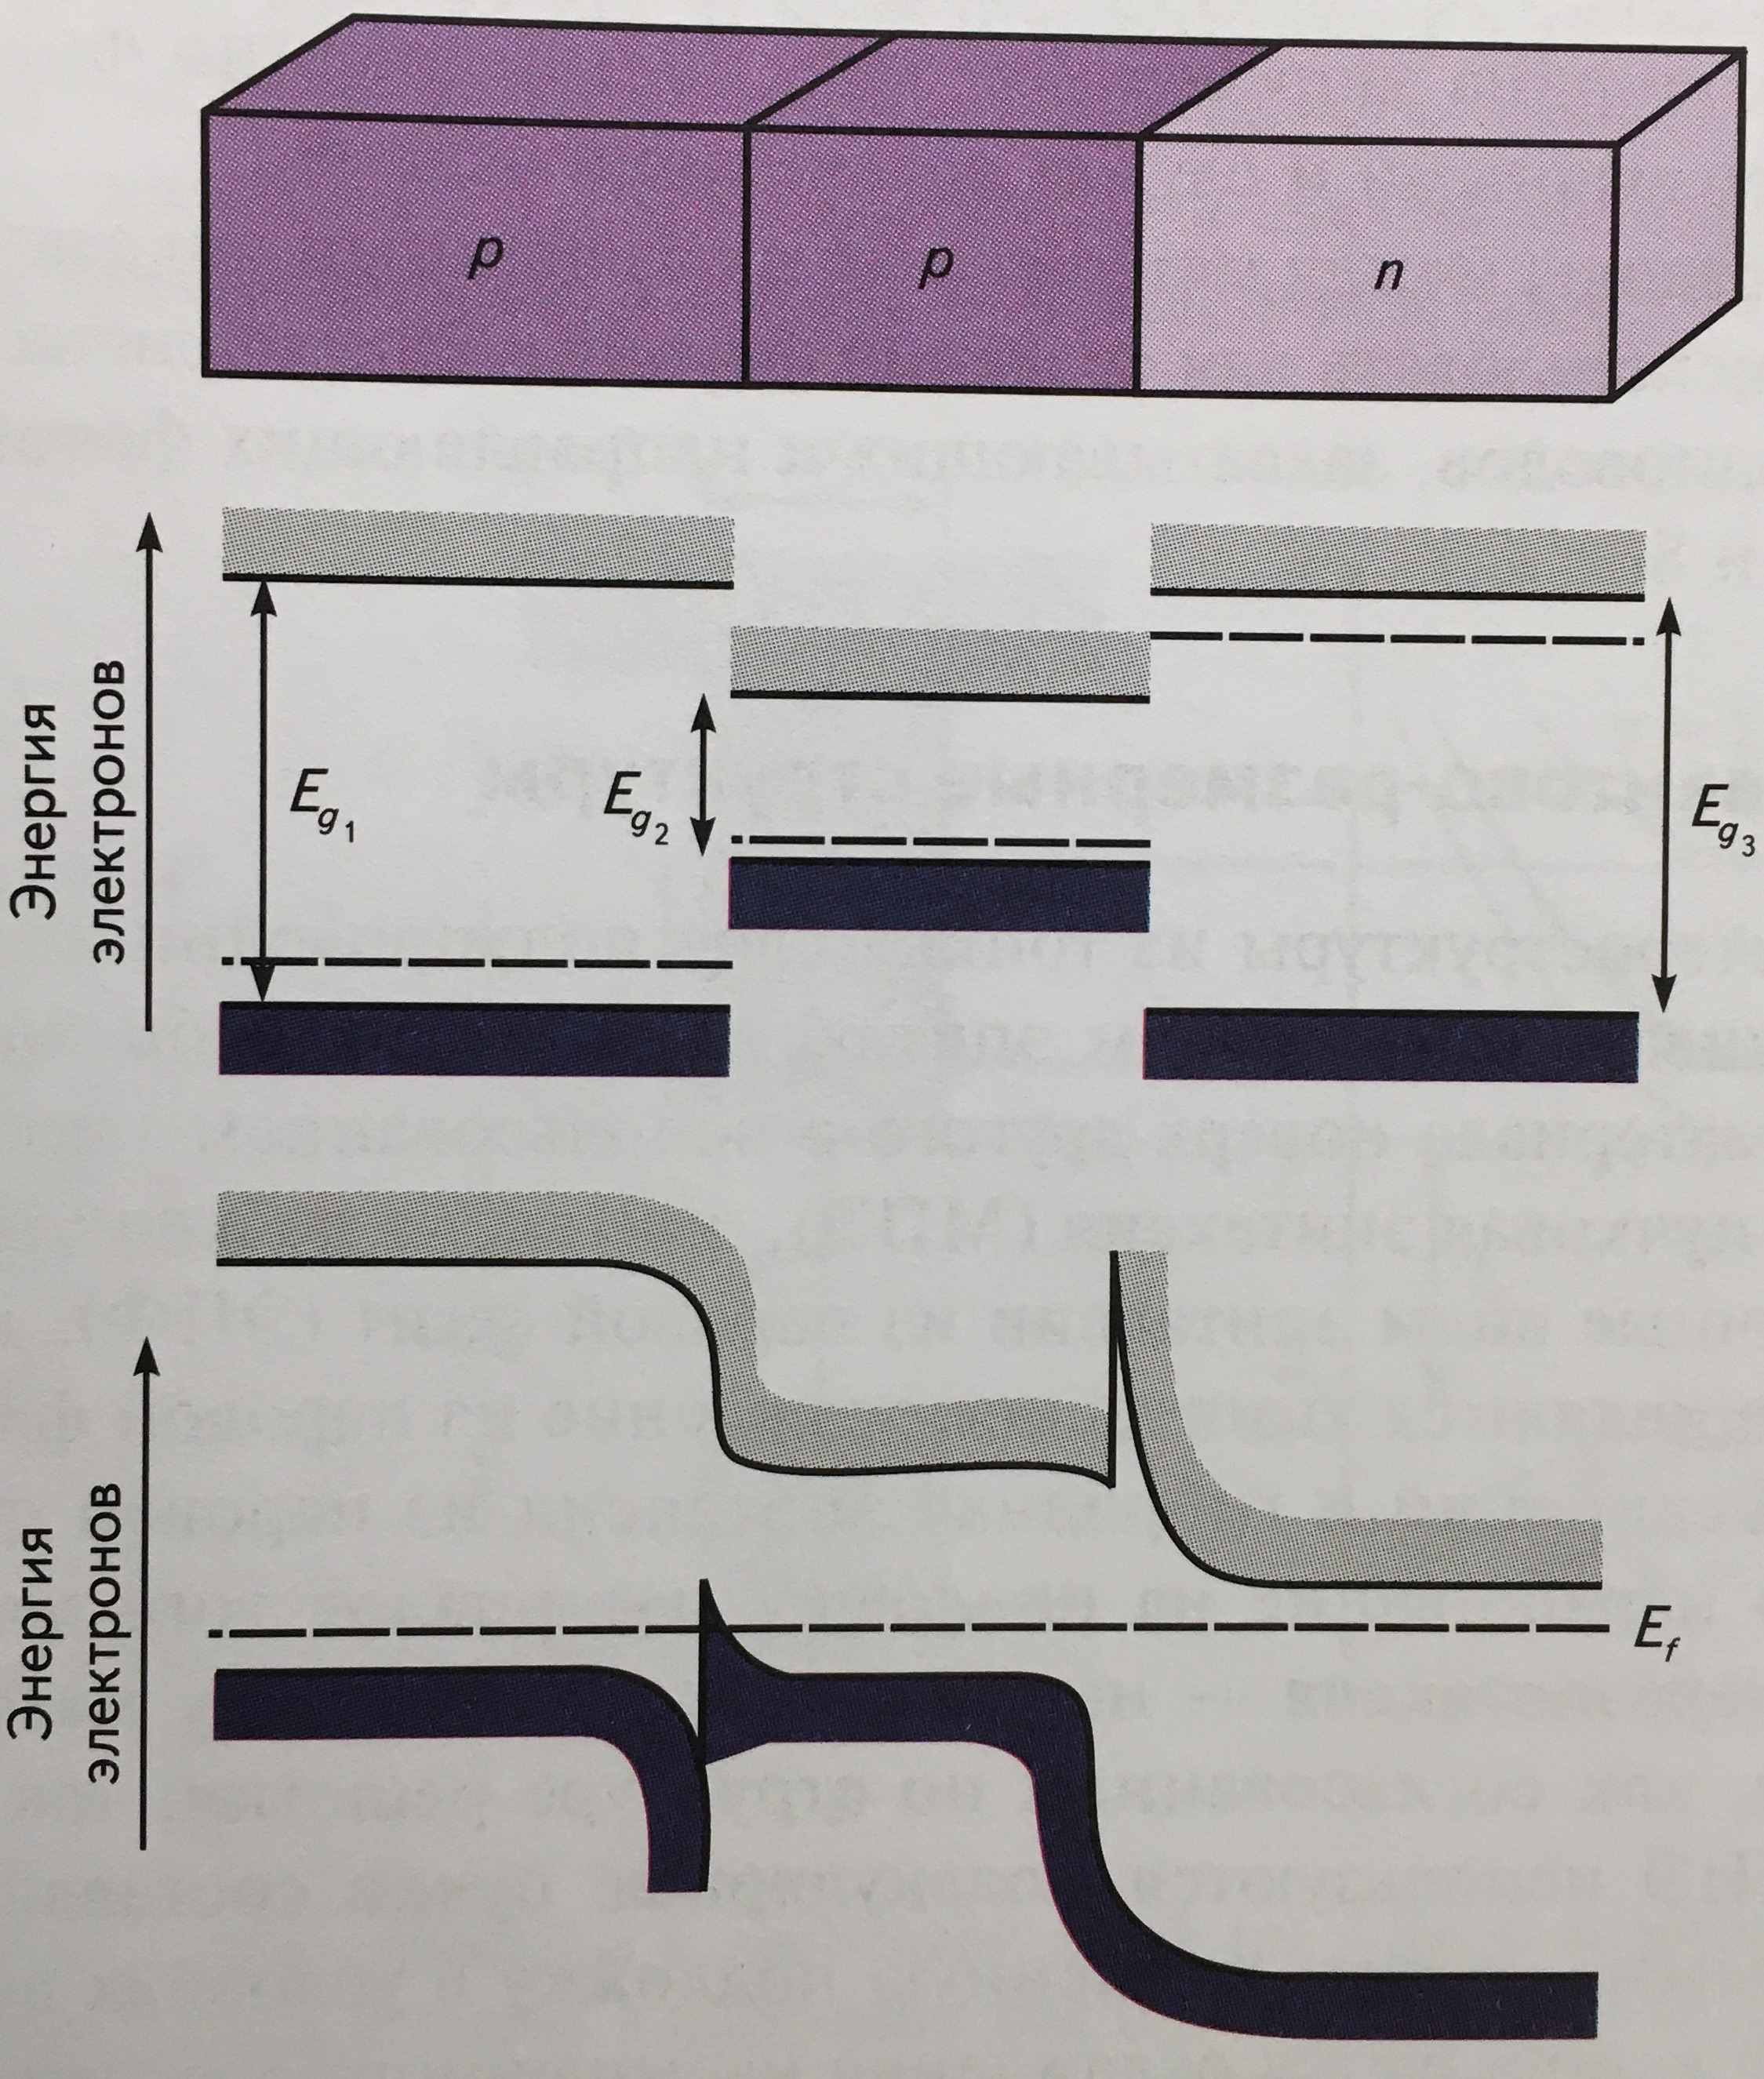
\includegraphics[width=0.5\linewidth]{8} 
    \caption{$p-p-n$-структура с двойной гетероинжекцией}
    \label{fig:8}
\end{figure}






\subsection{Условия поглощения и испускания}
Возбуждение электрона из валентной зоны в зону проводимости
возможно в результате поглощения фотона с соответствующей энергией
($h\nu>E_{g}$ или $\lambda < \lambda_{g}$). Рождается
электронно-дырочная пара. Это вносит добавку в концентрацию подвижных
носителей заряда и повышает электропроводность материала. Материал
ведет себя как фотопроводник с проводимостью, пропорциональной потоку
фотонов. Этот эффект используется для детектирования света.

Переход электрона из зоны проводимости в валентную зону
(электронно-дырочная рекомбинация) может иметь своим результатом
испускание фотона с энергией $h\nu > E_{g}$, причем либо спонтанное,
либо вынужденное, если фотон с такой энергией уже имеется. Спонтанное
излучение лежит в основе действия светоизлучающего диода. Вынужденное
излучение отвечает за работу полупроводниковых оптических оптических
усилителей и диодных лазеров. 

Условия, при которых происходит поглощение и испускание, можно
сформулировать следующим образом:
\begin{enumerate}
    \item \emph{Сохранение энергии}. Для поглощения или испускания
        фотона с энергией $h\nu$ требуется, чтобы энергии двух
        состояний, участвующих во взаимодействии (скажем, $E_{1}$ в
        валентной зоне и $E_{2}$ в $E_{2}$ в зоне проводимости) были
        разделены интервалом $h\nu$.
    \item \emph{Сохранение импульса}. Импульс также должен сохраняться
        в процессе испускания или поглощения фотона, так что
        \[
            p_{2}-p_{1}= \frac{h\nu}{c}= \frac{h}{\lambda}
            \hspace{1em} или \hspace{1em} k_{2}-k_{1}=
            \frac{2\pi}{\lambda}
        \]
        Однако величина импульса фотона $h/\lambda$ очень мала по
        сравнению с возможными значениями импульса электронов и дырок.
        Следовательно, импульсы электрона и дырки, участвующие во
        взаимодействии, должны быть приблизительно равны. Условие
        $k_{2}\approx k_{1}$ называется \emph{правилом отбора по k}. 
    \item \emph{Энергии и импульсы электрона и дырки, с которыми
        взаимодействует фотон}. Законы сохранения требуют, чтобы фотон
        с частотой $\nu$ взаимодействовал с электронами и дырками со
        специфическими значениями энергии и импульса, определяемыми
        соотношением между $E$ и $k$ для данного полупроводника. 
    \item \emph{Оптическая совместная плотность состояний}. Определим
        плотность состояний $\rho(\nu)$, с которым фотон с энергией
        $h\nu$ взаимодействует при выполнении условий сохранения
        энергии и импульса в прямозонном проводнике. Эта величина
        включает плотности состояний как в валентной зоне, так и в
        зоне проводимости и называется \emph{оптической совместной
        плотностью состояний}. 
\end{enumerate}


\begin{figure}[H]
    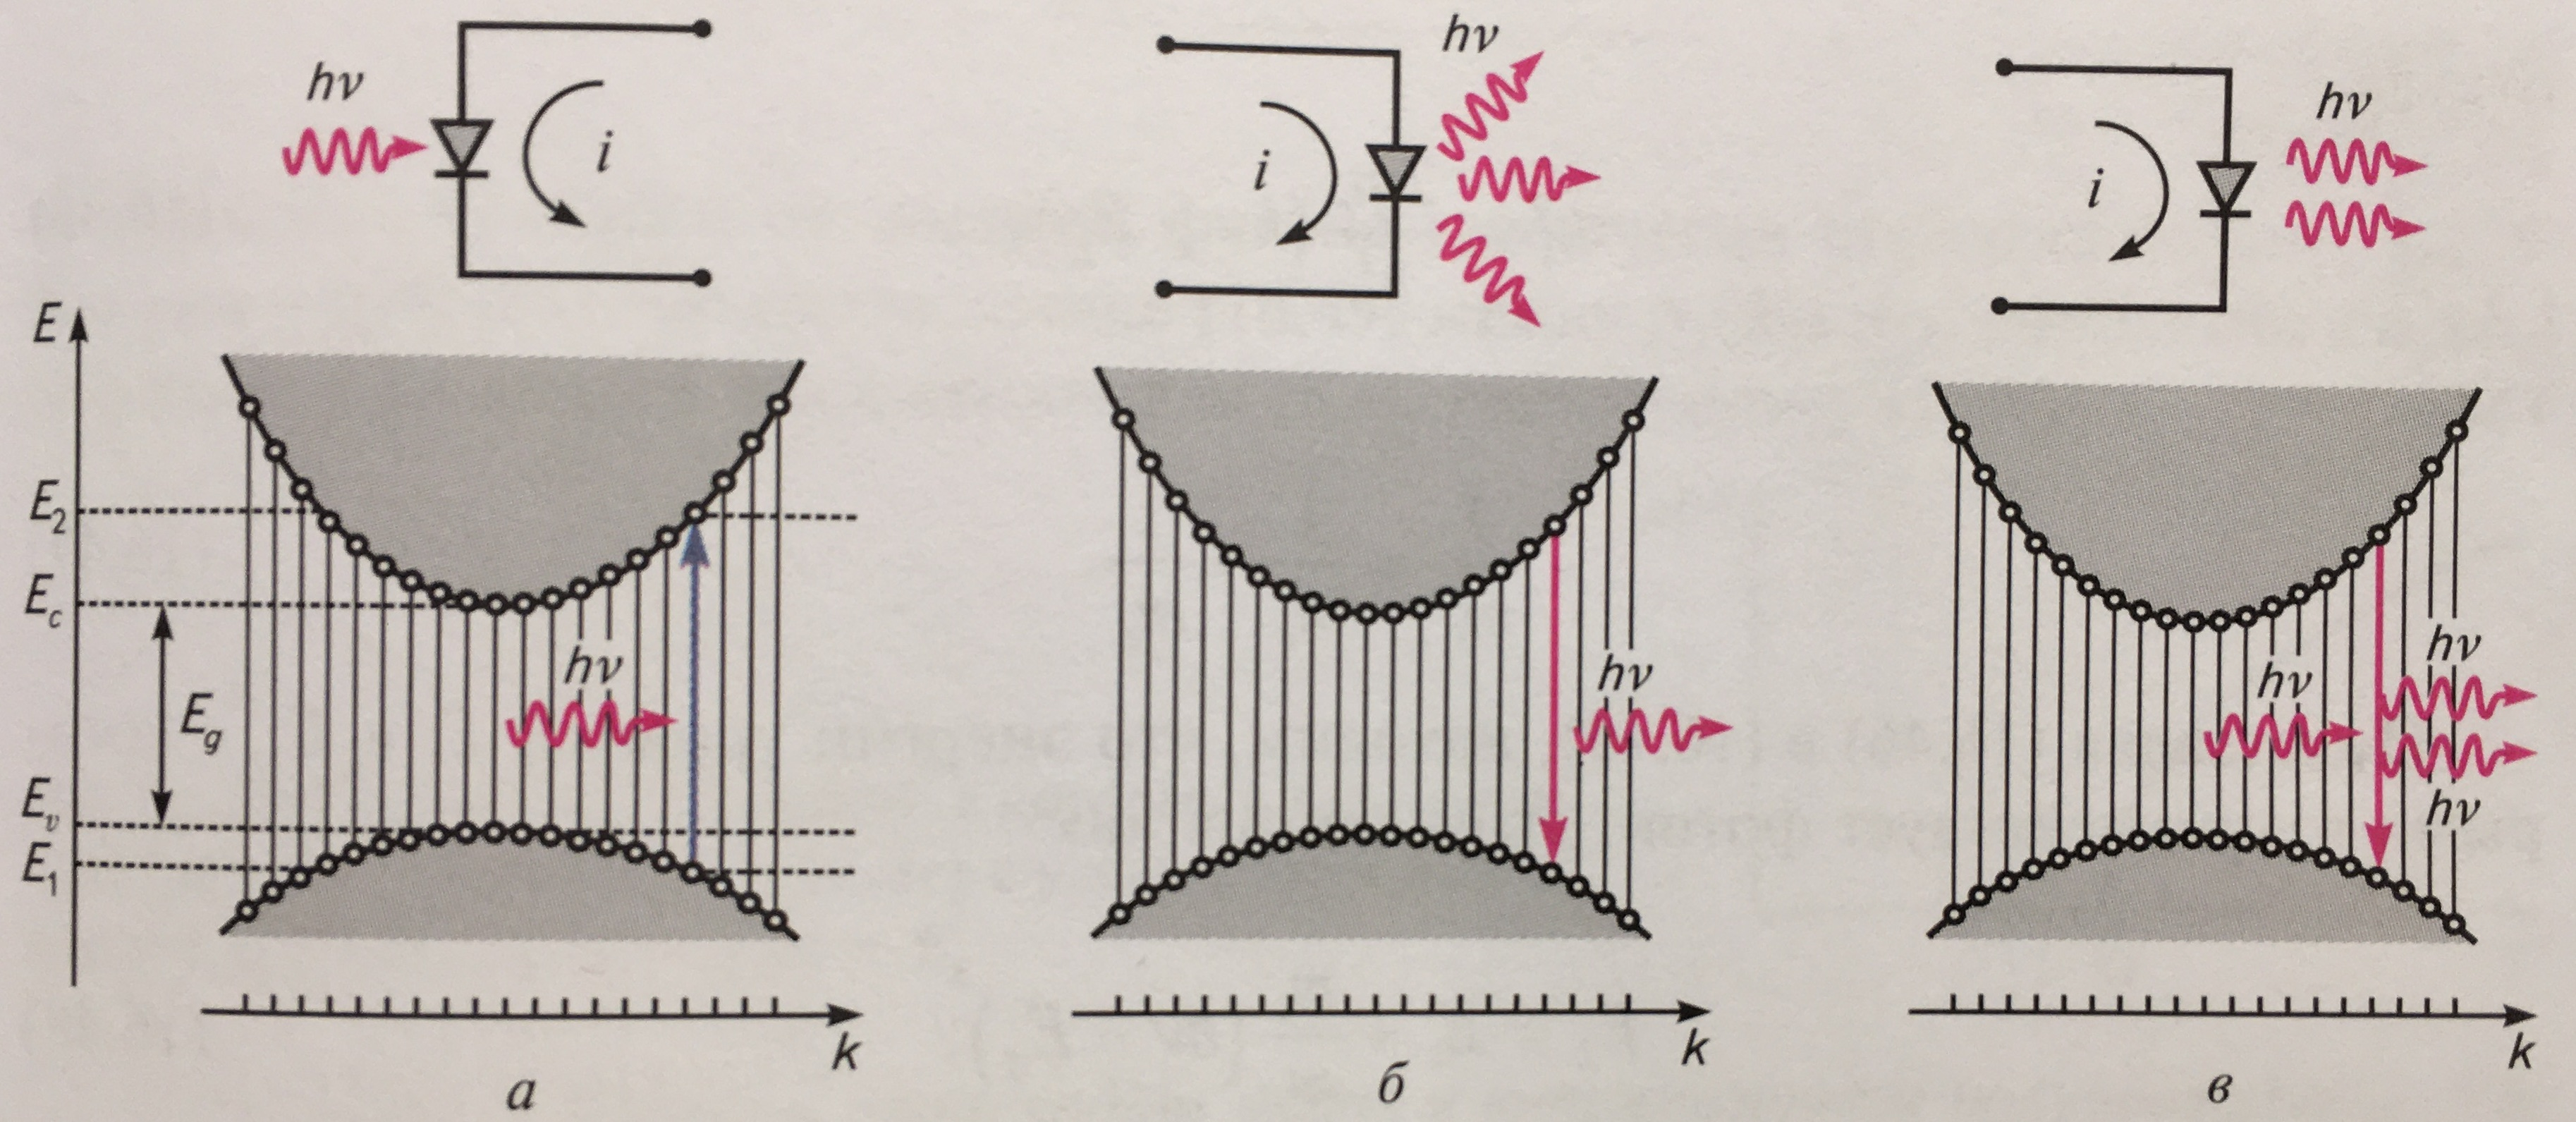
\includegraphics[width=0.7\linewidth]{9} 
    \caption{Поглощение фотона приводит к рождению электронно-дырочной
    пары. Процесс используется в фотоприемниках (а). Рекомбинация
электронно-дырочной пары сопровождается спонтанным испусканием фотона
(б). На этой основе работают светоизлучающие диоды. Рекомбинация
электрона и дырки может быть индуцирована фотонов (в). В результате
происходит вынужденное испускание идентичного фотона. Этот процесс
лежит в основе действия полупроводниковых диодных лазеров}
\label{fig:9}
\end{figure}


\subsection{Светоизлучающие диоды}
Электролюминесценция --- это явление, при котором свет излучается
материалом под действием электроического поля. Инжекционная
электролюминесценция лежит в основе действия светоизлучающих диодов
--- высокоэффективных устройств, способных излучать свет любого цвета. 

Электронно-дырочкая радиационная рекомбинация приводит к излучению
света полупроводниковым материалом. Однако при комнатной температуре
тепловая концентрация электронов и дырок так низка, что возникающий
поток фотонов очень мал.

Скорость испускания фотонов можно существенно увеличить с помощью
внешних воздействий, увеличивающих избыточную концентрацию
электронно-дырочных пар в материале. Это можно осуществить, например,
освещая материал светом, но, как правило, это достигается помощью
смещения диода на $p-n$-переходе, которое способствует инжекции
носителей в область перехода.

\subsection{Полупроводниковые лазеры}
Принципы, на которых основано действие полупроводниковых лазерных
усилителей (ПОУ --- полупроводниковые оптические усилители), те же
самые, что и у других лазерных усилителей: создание
инверсии заселенностей приводит к преобладанию вынужденного испускания
над поглощением. Инверсия заселенностей обычно создается током
инжекции через $p-n$-переход в диоде; прямое напряжение смещения
вызывает инжекцию пар носителей в область перехода, где они
рекомбинируют посредством вынужденного испускания фотонов. 

Для целей сравнения ПОУ можно рассматривать как четырехуровневую
лазерную систему, у которой верхние два уровня лежат в зоне
проводимости, а нижние два --- в валентной зоне.


\begin{figure}[H]
    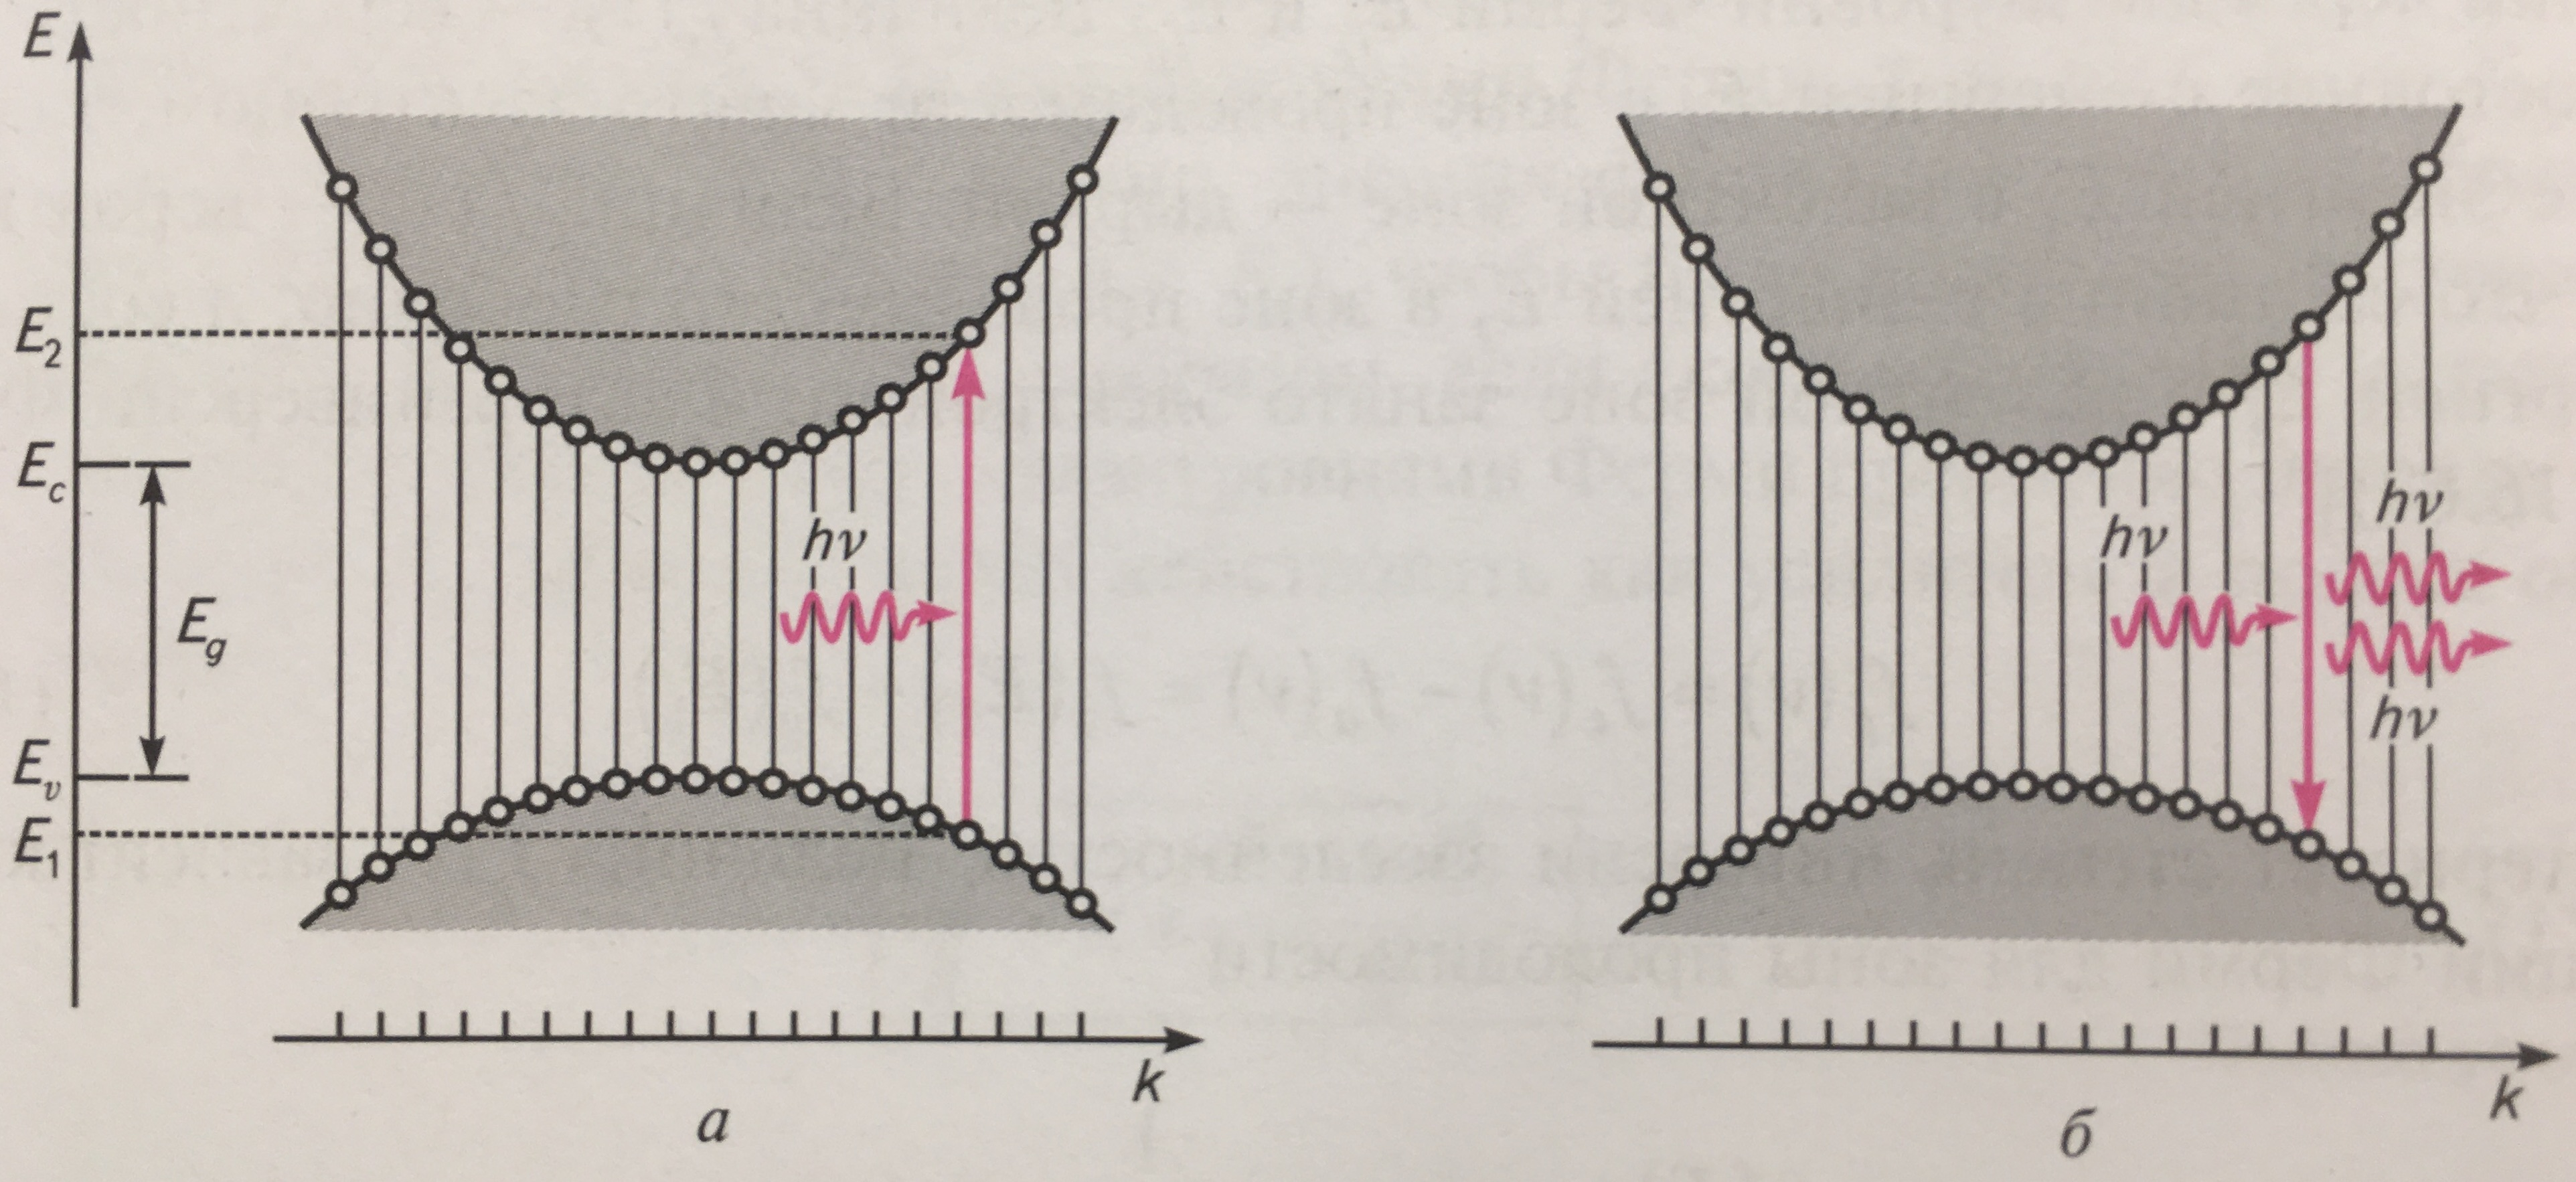
\includegraphics[width=0.8\linewidth]{15} 
    \caption{Поглощение фотона приводит к рождению электронно-дырочной
    пары (а). Рекомбинация электрона и дырки может быть индуцирована
фотоном; в результате происходит вынужденное испускание точно такого
же фотона (б)}
\label{fig:15}
\end{figure}

Свет частоты $\mu$ может взаимодействовать с носителями заряда
полупровдникововм материале с шириной запрещенной зоны $E_{g}$ за счет
межзонных переходов, при условии что $\mu > E_{g}/h$. Падающие фотоны
могут быть поглощены с рождением электронно-дырочной пары либо
вызывать рождение новых фотонов путем вынужденной рекомбинации
электрона и дырки. Когда испускание становится более вероятным, чем
поглощение, материал может служить когерентным оптическим усилителем.




\section{Оборудование}
В работе используются синий, красный, желтый, зеленый, белый
светодиоды, лазерный диод на $840~нм$, монохроматор МДР-23.

В монохроматоре для исследования спектра в области $0,8-0,9\: мкм$
($800-900\: нм$) установлена дифракционная решетка $600$ штрихов/мм с
максимальной концентрацией энергии в области $1\: мкм$. Обратная
линейная дисперсия монохроматора с этой решеткой равна $2,6\: нм/мм$.
Сканирование спектра реализуется с помощью шагового двигателя, который
осуществляет поворот дифракционной решетки. Питание шагового двигателя
осуществляется от выносного блока. Свет от лазерного диода с помощью
коденсора фокусируется на входную щель монохроматора. После
монохроматора сигнал попадает на обработку в компьютер. 


\begin{figure}[H]
    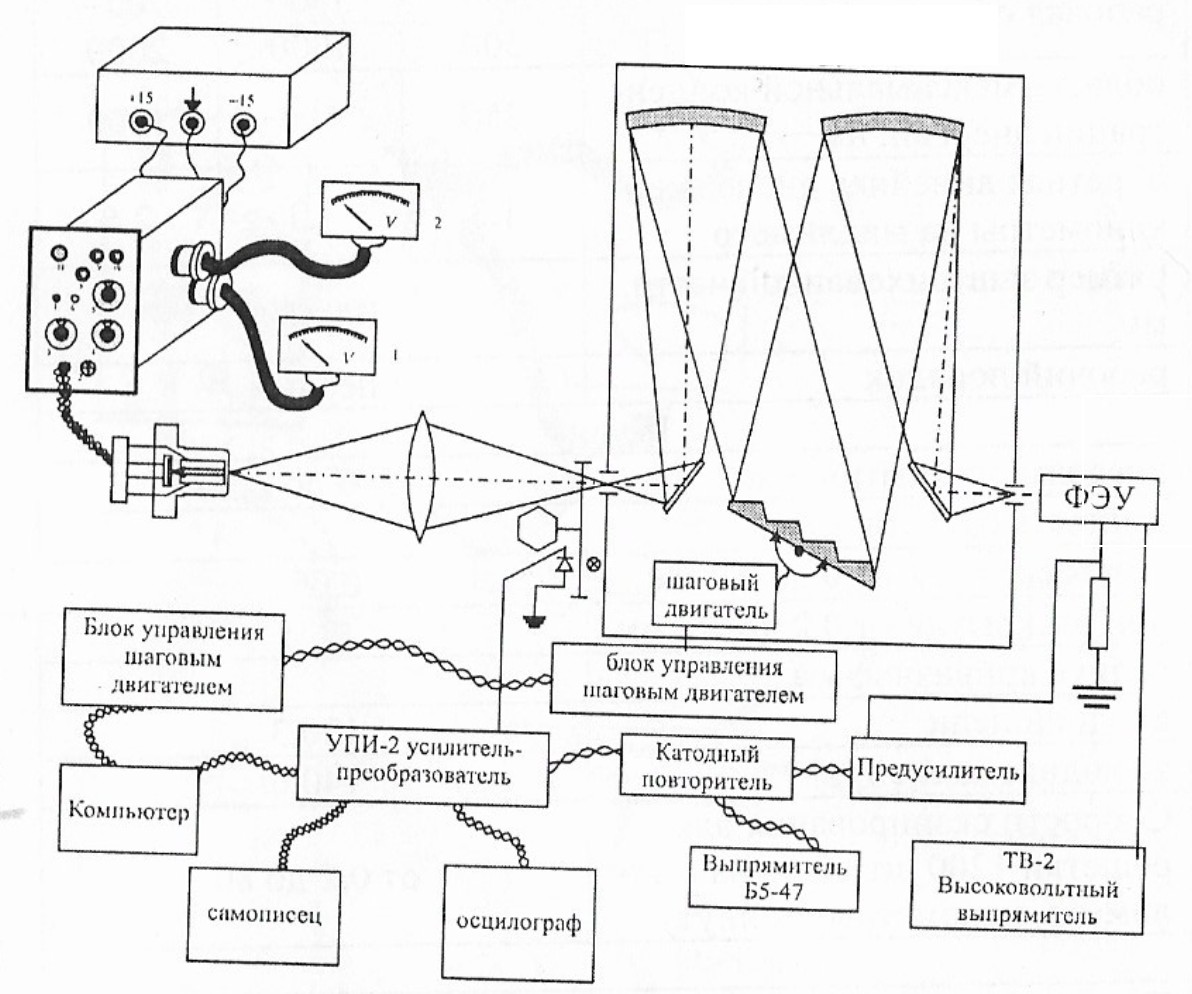
\includegraphics[width=0.8\linewidth]{10} 
    \caption{Установка для исследования спектрального состава
    излучения полупроводникового лазер}
    \label{fig:10}
\end{figure}





\section{Результаты измерений и обработка результатов}
Снимем ВАХ всех светодиодов. 

\begin{figure}[H]
    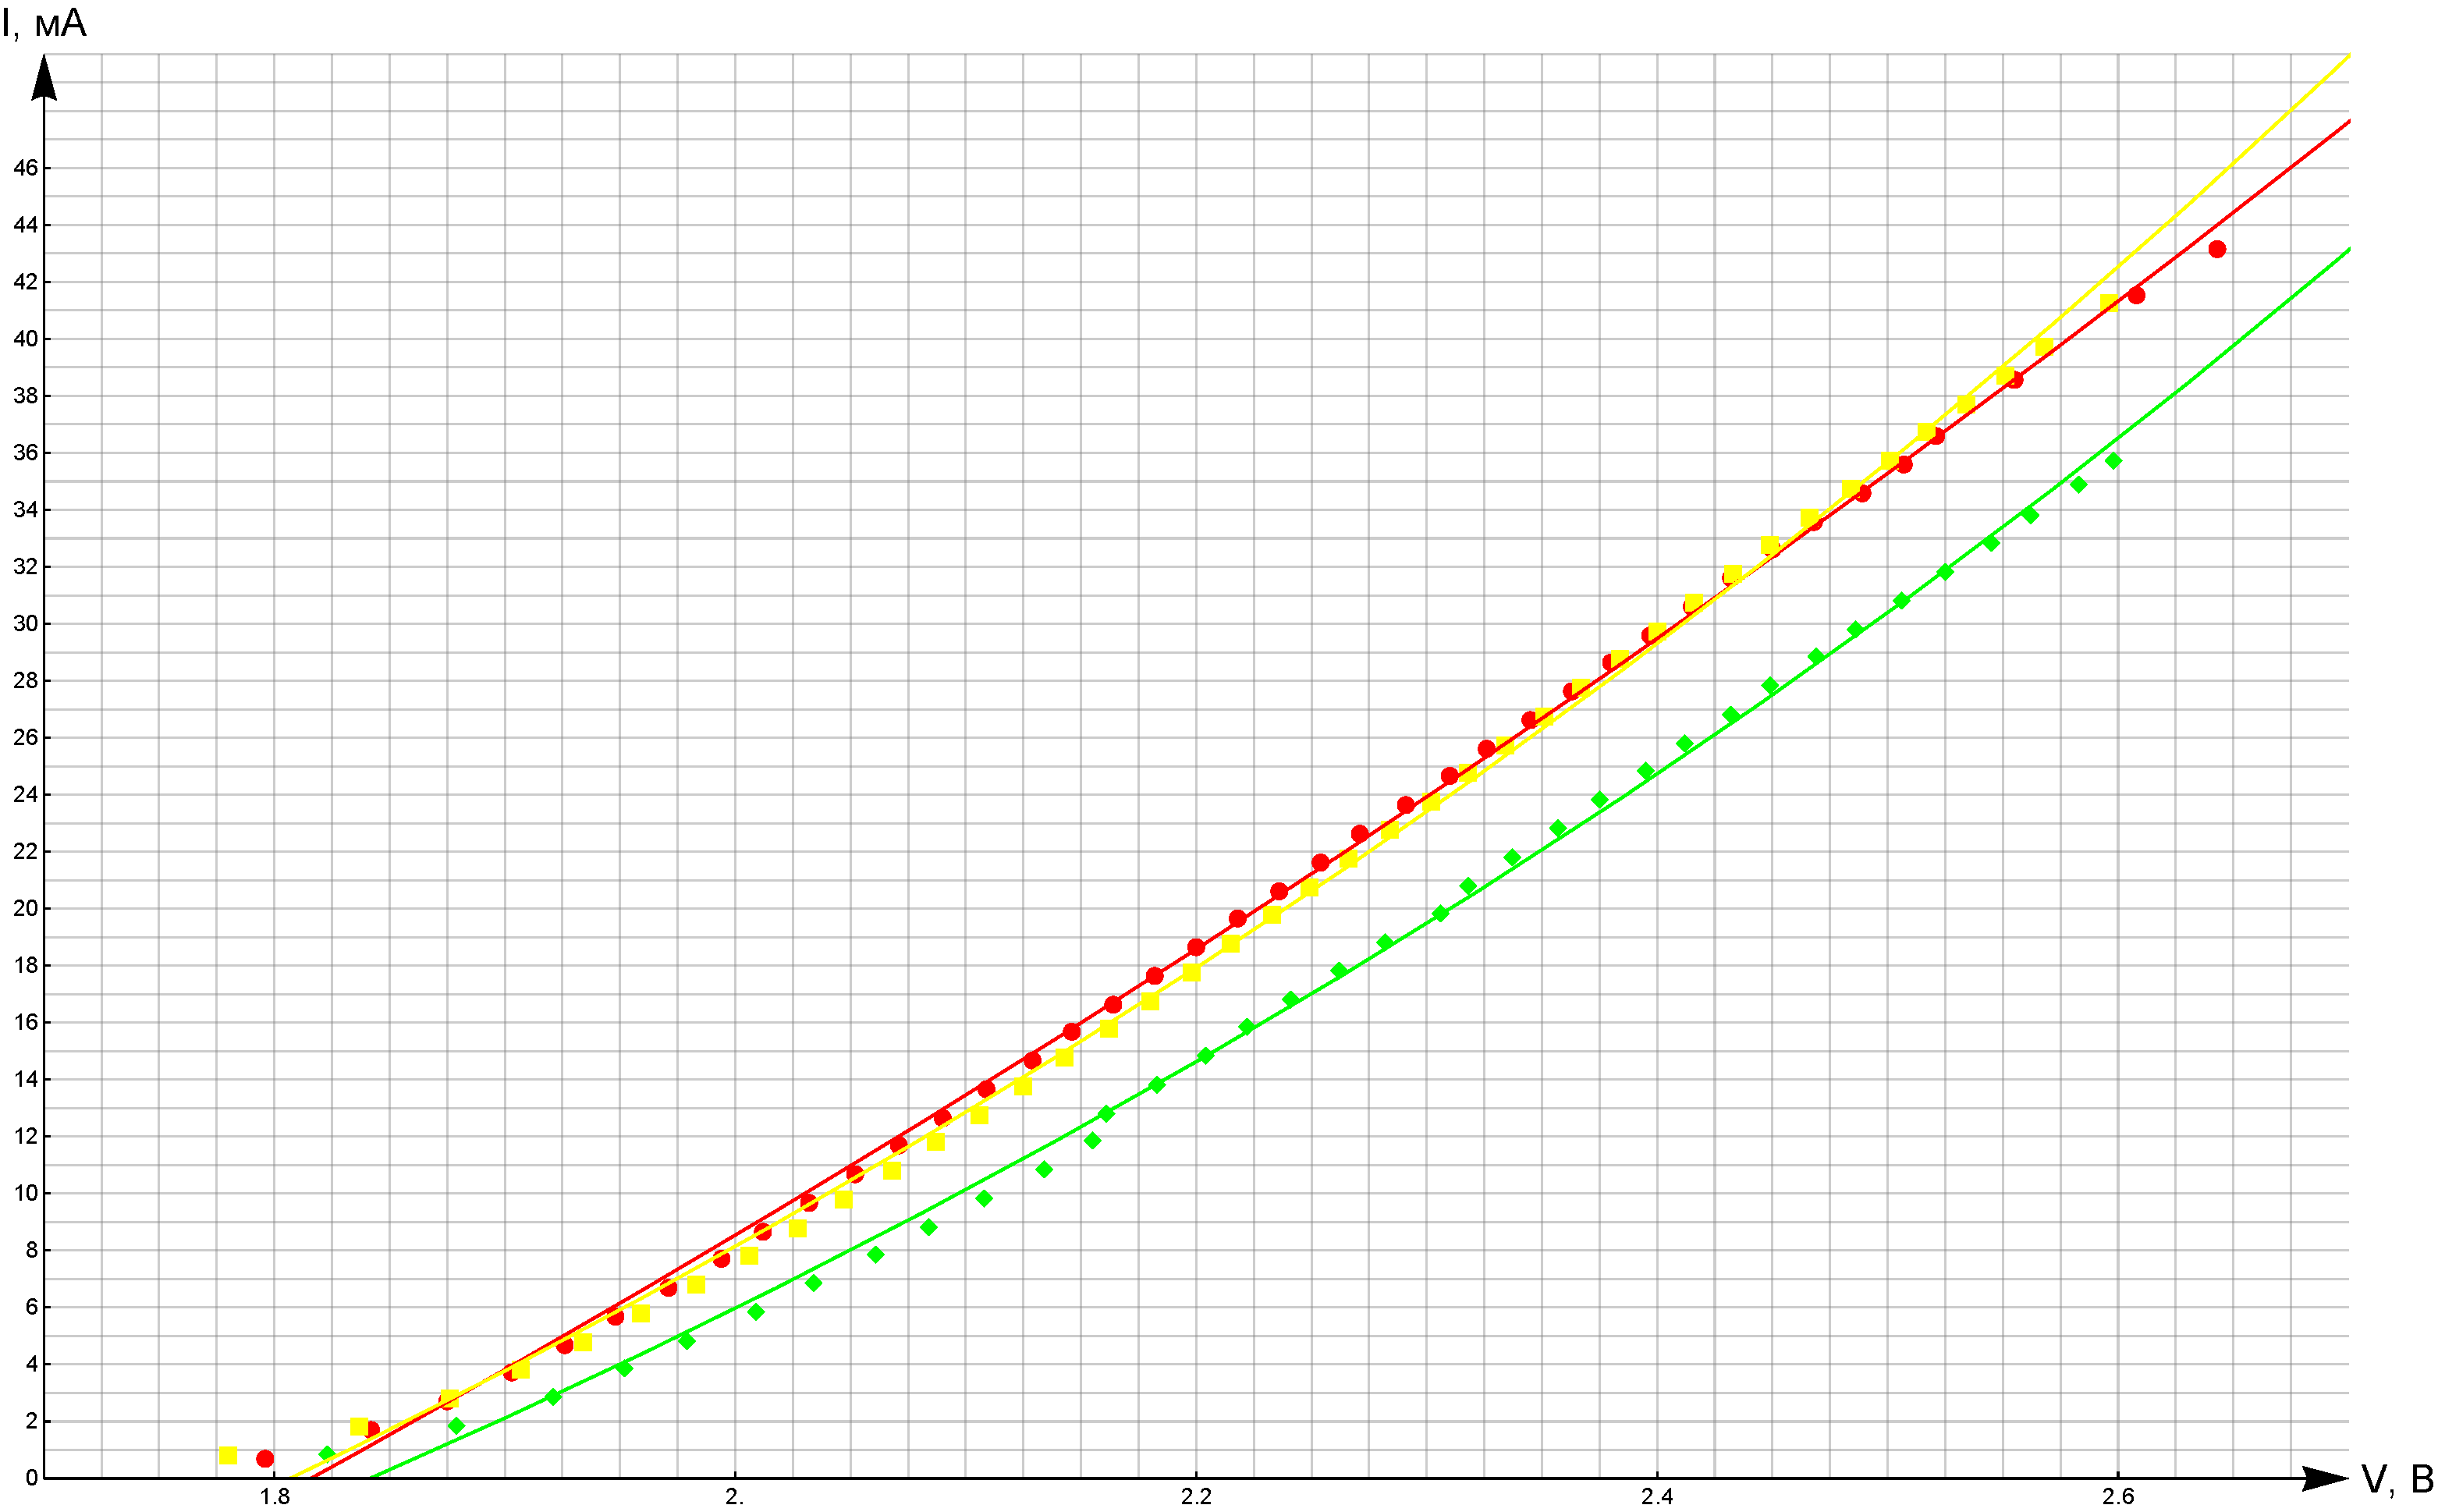
\includegraphics[width=0.8\linewidth]{11} 
    \caption{Вольт-амперная характеристика красного, желтого, зеленого 
    светодиодов}
    \label{fig:11}
\end{figure}

\begin{figure}[H]
    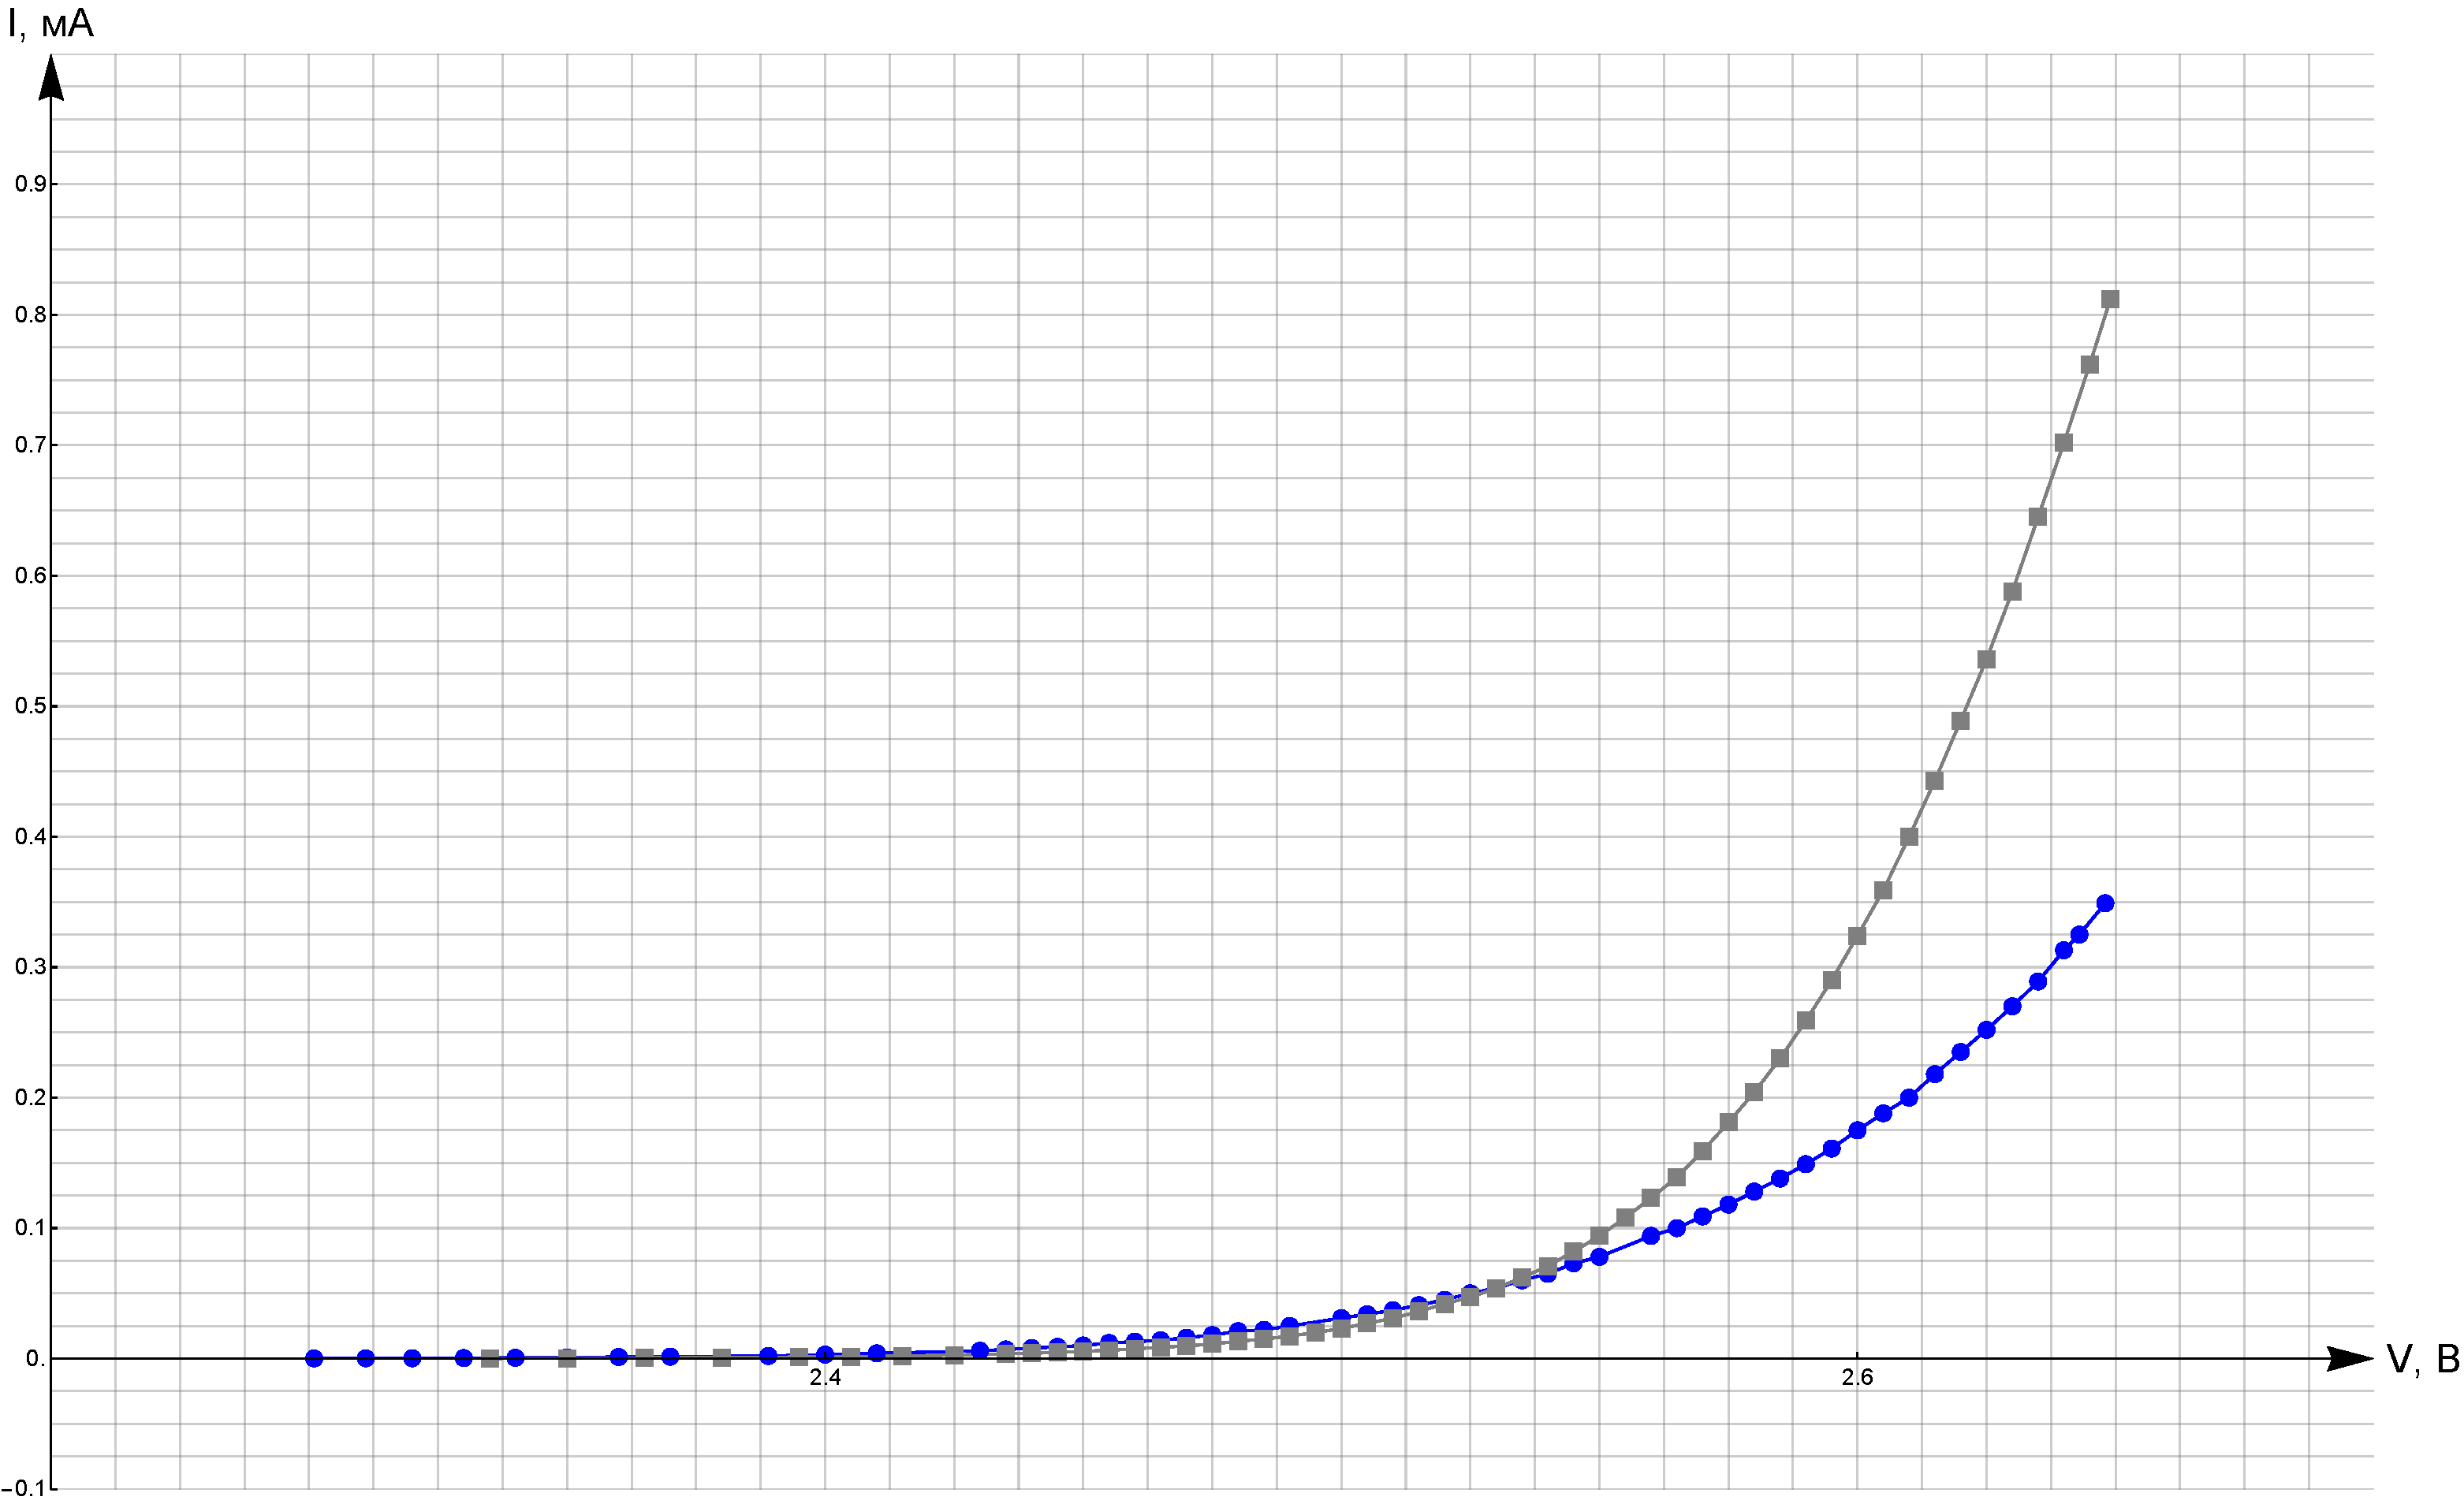
\includegraphics[width=0.8\linewidth]{12} 
    \caption{Вольт-амперная характеристика белого и синего
    светодиодов}
    \label{fig:12}
\end{figure}

Снимем спектр красного светодиода, собрав установку на \fig{fig:10} 

\begin{figure}[H]
    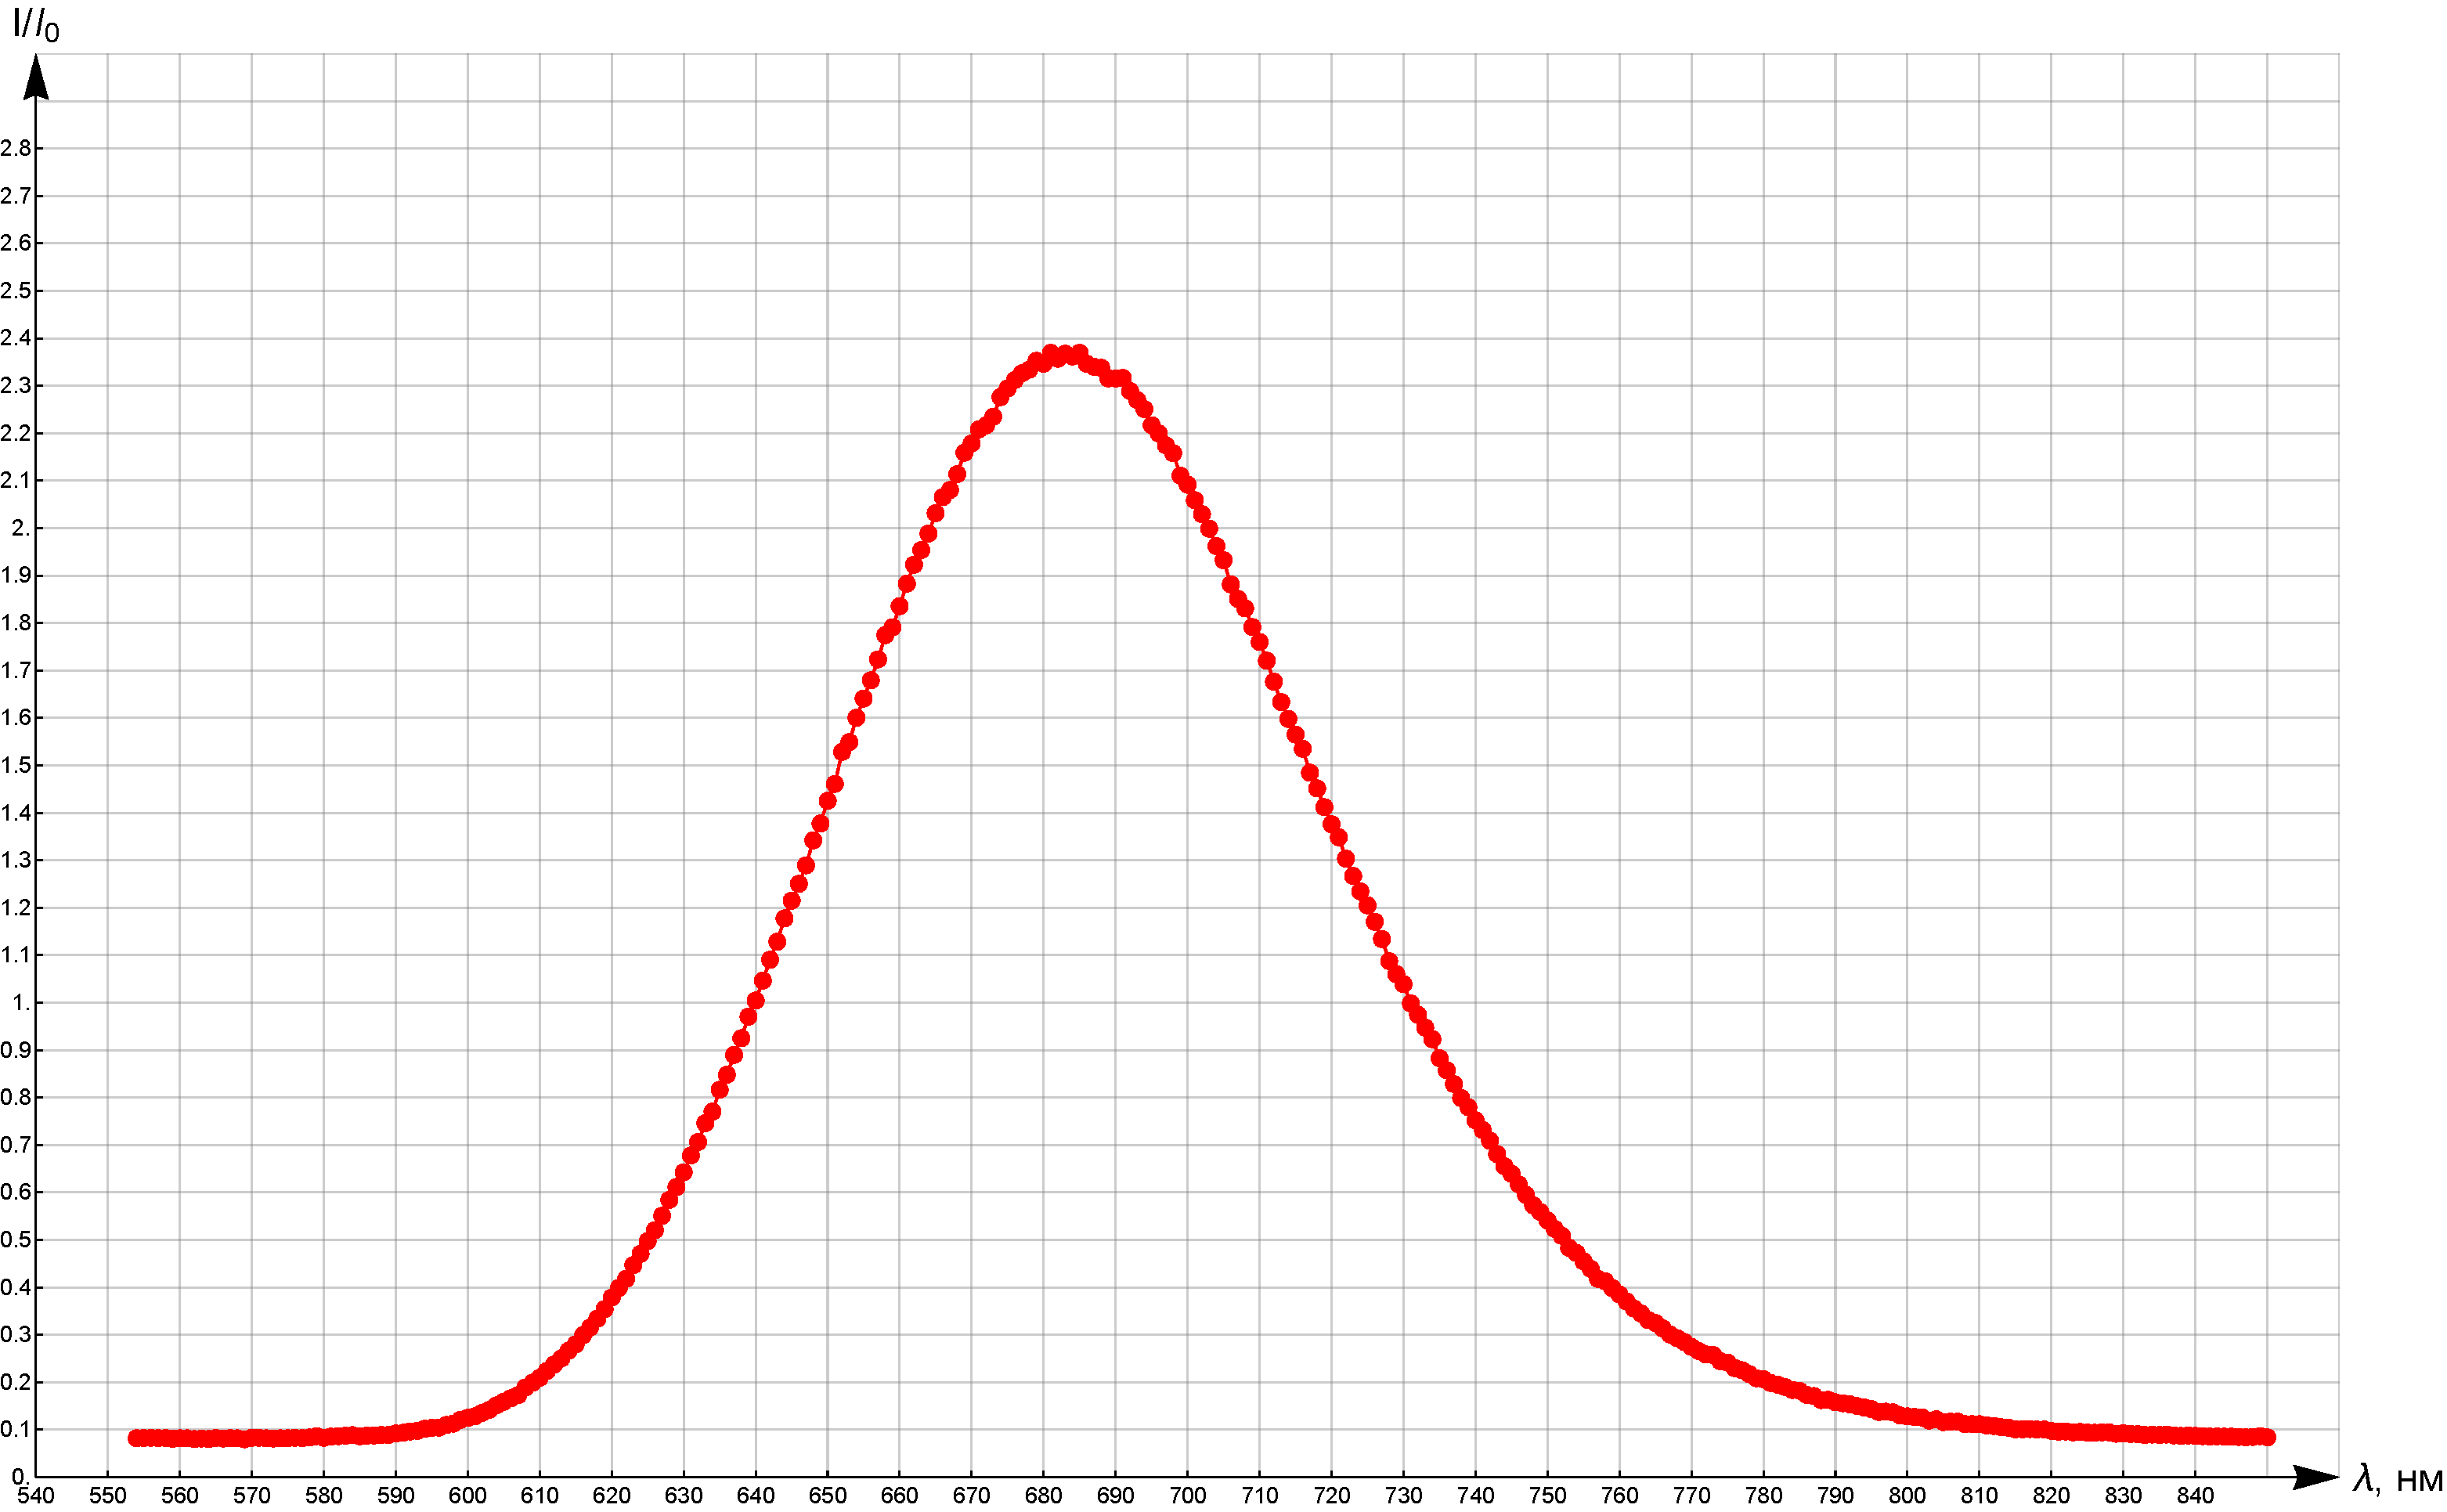
\includegraphics[width=0.8\linewidth]{13} 
    \caption{Спектр красного светодиода}
    \label{fig:13}
\end{figure}


Снимем спектр лазерного диода с модовой структурой

\begin{figure}[H]
    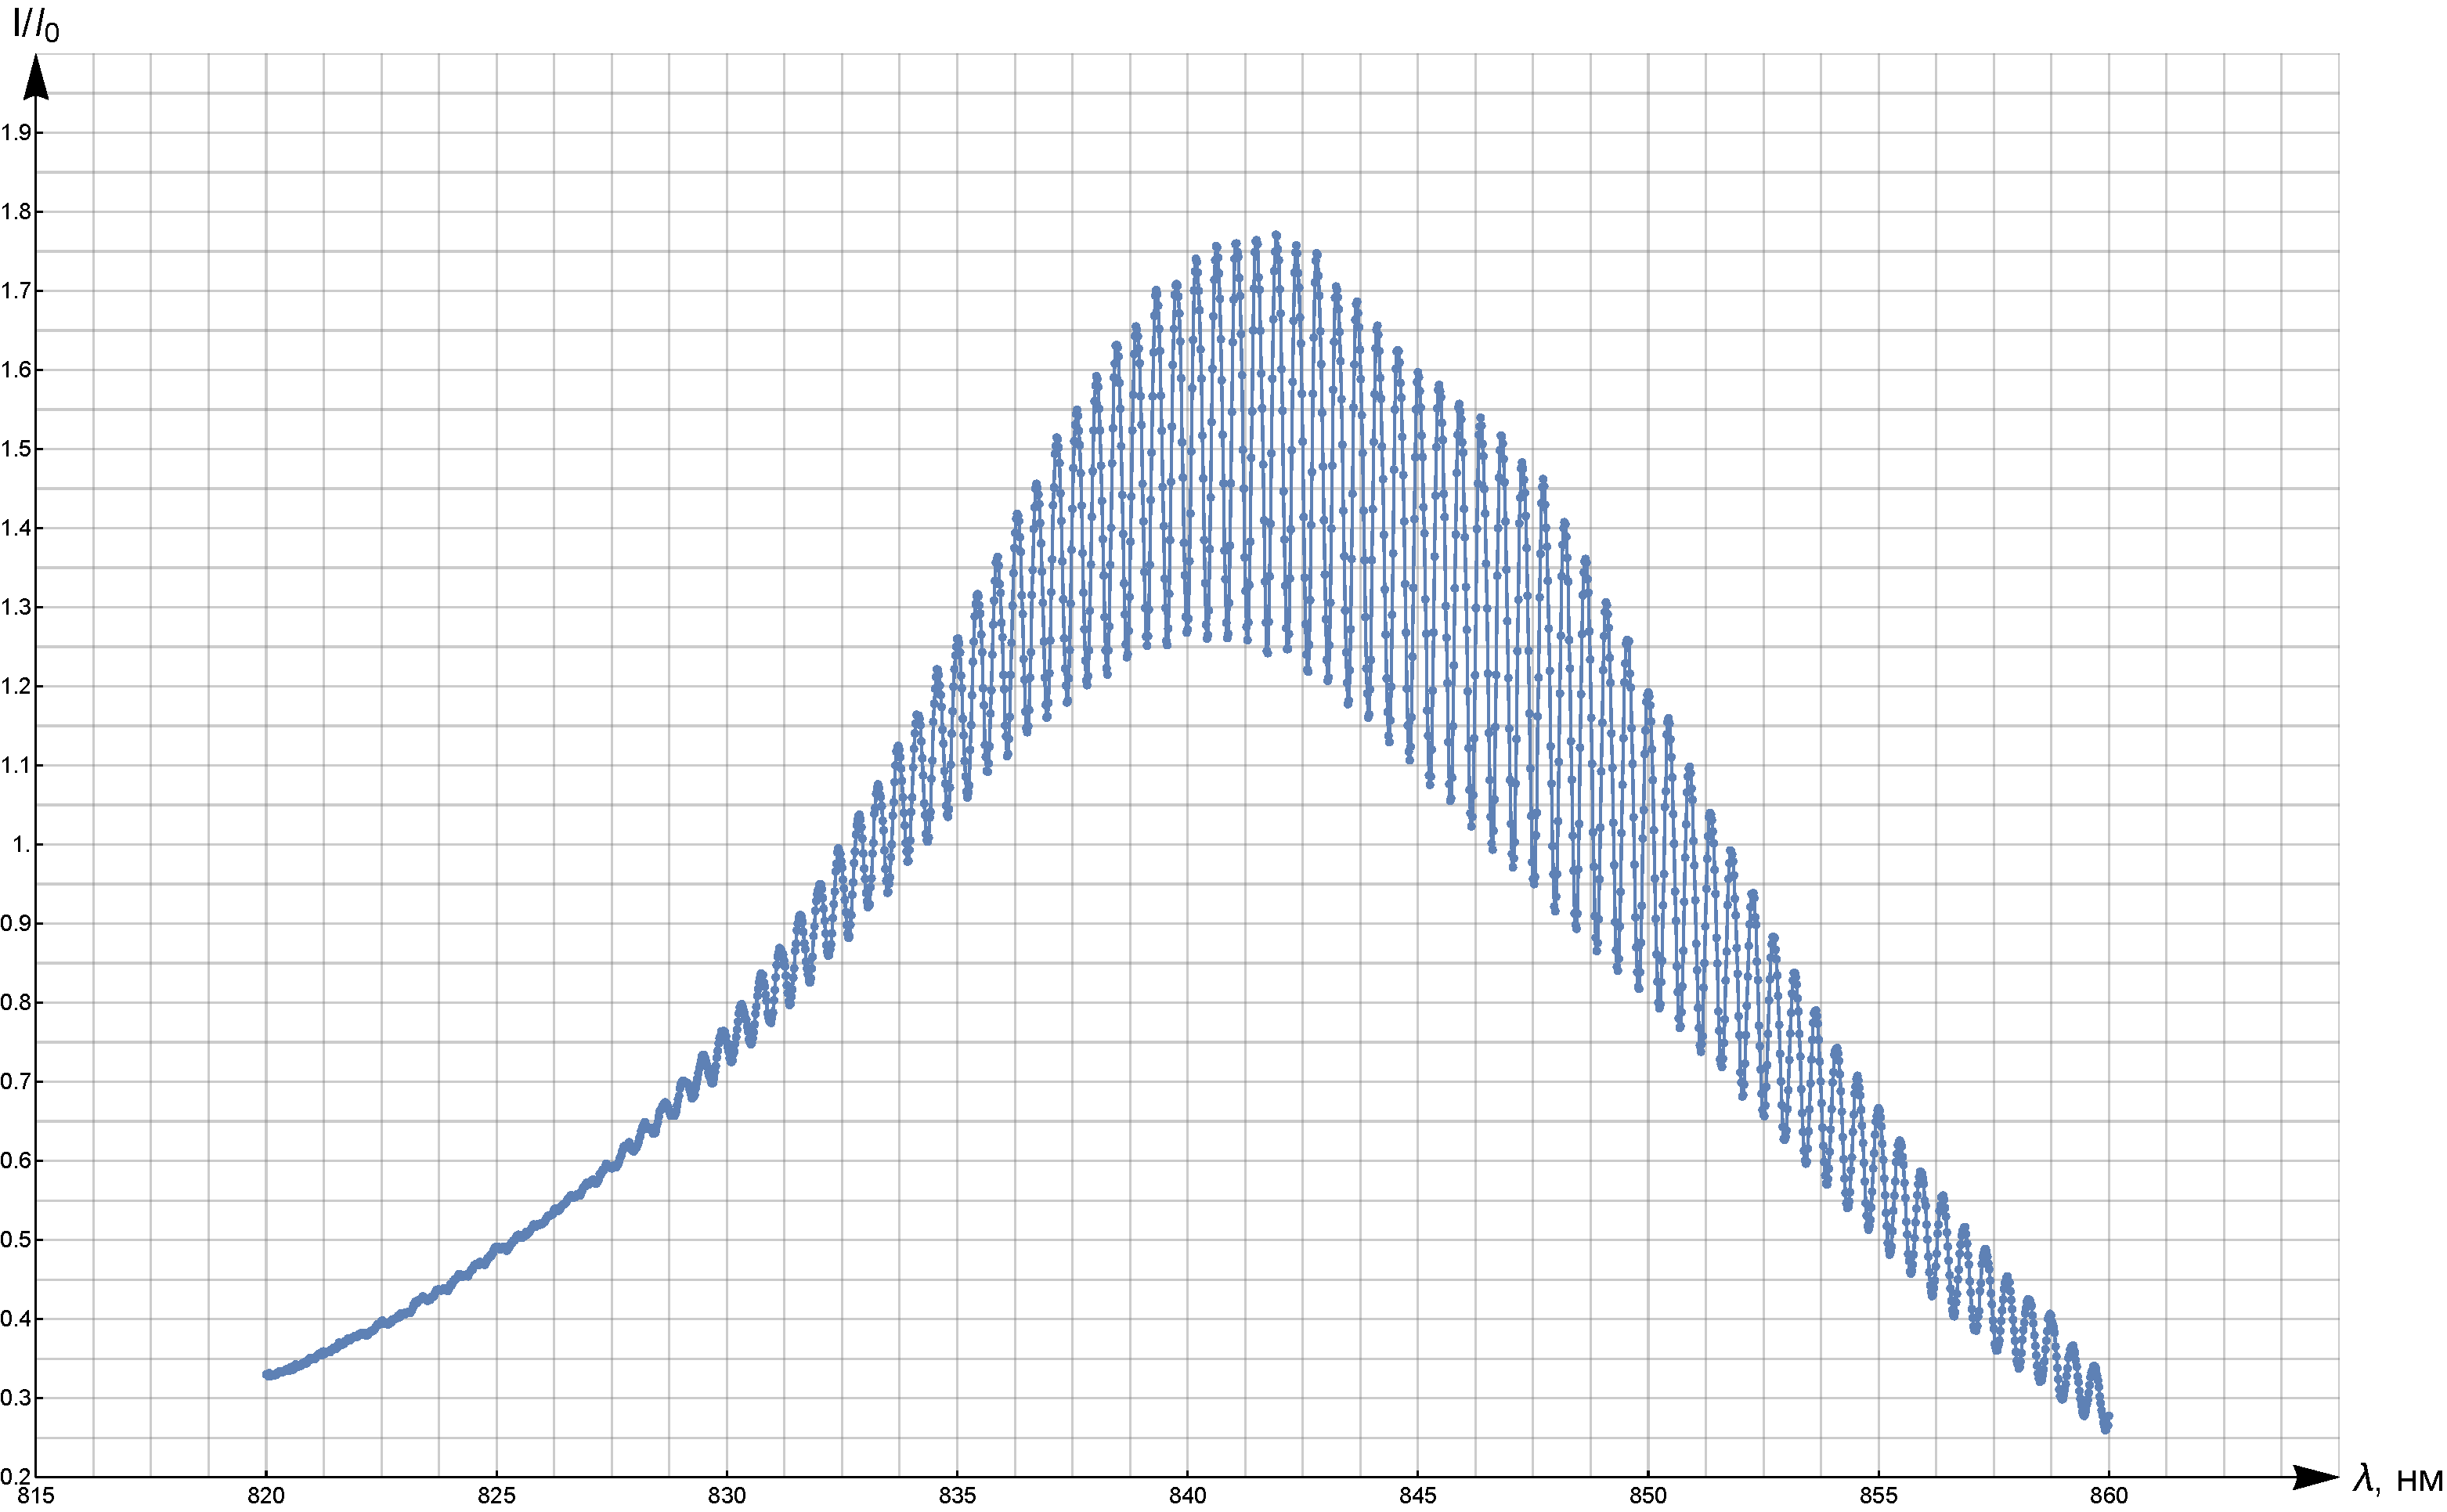
\includegraphics[width=0.8\linewidth]{14} 
    \caption{Спектр полупроводникового лазера с модовой структурой}
    \label{fig:14}
\end{figure}

Посчитаем по спектру с модовой структурой длину резонатора лазера $d$.
Запишем условие резонанса:
\begin{equation*}
    \begin{gathered}
        d=\lambda m = (\lambda + \Delta \lambda)(m-1)\\
        m= \frac{\lambda}{\Delta \lambda}+1
    \end{gathered}
\end{equation*}

Из спектра $\Delta lambda \approx 0,44\: нм$, откуда получаем $m$:
\[
    m\approx 1915
\]

И в итоге получаем $d$:
\[
    d\approx 1,6\: мм
\]







\section{Обсуждение результатов и выводы}
Рассмотрены принципы работы полупроводниковых источников света ---
светодиодов и лазеров.

Были получены вольт-амперные характеристики светодиодов
(\fig{fig:11}, \fig{fig:12}), спектр красного светодиода
\ffig{fig:13} и спектр полупроводникового лазера с модовой структурой
\ffig{fig:14}.

Вольт-амперные характеристики хорошо аппроксимируются уравнением Шокли
\eqref{eq:diod}.

По ширине спектра можно сделать вывод, что спектр полупроводникого
лазера гораздо уже спектра светоизлучающего диода за счет вынужденного
излучения.

Стоит отметить некоторые преимущества полупроводниковых лазеров и их
применение в промышленности. Первой характерной особенностью является,
что такие лазеры имеют широкие и интенсивные полосы поглощения, это
подразумевает главным образом использование оптической накачки.
Высокие значения коэффициента поглощения допускают использование
лазеров с размерами до нескольких микрон. Второй важной характерной
особенностью является то, что эти активные среды имеют широкую полосу
люминесценции и, следовательно, широкую полосу усиления. С одной
стороны, это предполагает перестройку частоты генерации в широком (до
нескольких нанометров) диапазоне. С другой стороны, эта особенность
позволяет генерировать импульсы с очень малой длительностью
(фемтосекундные импульсы) в режиме синхронизации мод. Третья
характерная особенность заключается в том, что эффективность
преобразования (при оптической накачке для твердотельных среда и
красителей и электрической накачке для полупроводников) в упомянутых
лазерах обычно достаточно велика. 

Маломощные ($P=5-20\: мВт$) однополосковые лазеры широко используются
в проигрывателях компакт-дисков и в лазерных принтерах. Более мощные
однополосковые лазеры, лазерные линейки, лазерные матрица и массивы из
лазерных линеек используются для накачки твердотельных активных сред.










\end{document}
